% =============================================================================
% Arquitectura de Codigo del Simulador de Pensiones
% Documento 3 de 4 -- Serie de Referencia Tecnica
% =============================================================================
\documentclass[11pt, letterpaper, twoside]{report}

% --- Paquetes fundamentales ---
\usepackage[utf8]{inputenc}
\usepackage[T1]{fontenc}
% babel spanish requires texlive-lang-spanish; using manual overrides instead
\usepackage{babel}
\renewcommand{\contentsname}{Contenido}
\renewcommand{\chaptername}{Cap\'{i}tulo}
\renewcommand{\tablename}{Tabla}
\renewcommand{\figurename}{Figura}
\renewcommand{\listfigurename}{Lista de Figuras}
\renewcommand{\listtablename}{Lista de Tablas}
\usepackage{lmodern}
\usepackage{microtype}

% --- Matematicas ---
\usepackage{amsmath}
\usepackage{amssymb}

% --- Geometria y layout ---
\usepackage[
  top=2.5cm,
  bottom=2.5cm,
  left=3cm,
  right=3cm,
  headheight=15pt
]{geometry}

% --- Colores (Tropical Vibrant) ---
\usepackage{xcolor}
\definecolor{teal}{HTML}{0f766e}
\definecolor{tealdark}{HTML}{115e59}
\definecolor{magenta}{HTML}{db2777}
\definecolor{pinklight}{HTML}{ec4899}
\definecolor{bodybg}{HTML}{fef7ed}
\definecolor{surface}{HTML}{fffbf0}
\definecolor{textmain}{HTML}{1e293b}
\definecolor{goldmuted}{HTML}{c4a67a}
\definecolor{bluebox}{HTML}{1e40af}
\definecolor{greenbox}{HTML}{065f46}
\definecolor{orangebox}{HTML}{c2410c}

% --- Listados de codigo ---
\usepackage{listings}
\lstdefinelanguage{R}{
  keywords={function, if, else, return, for, while, in, NULL, TRUE, FALSE,
            list, c, paste0, max, min, floor, ceiling, round, abs, as.numeric,
            as.character, as.Date, is.null, is.na, nrow, which, names, length,
            data.frame, rbind, order, switch, sapply, all,
            library, source, read.csv,
            reactive, reactiveVal, observe, observeEvent, isolate, req,
            debounce, renderUI, renderPlotly, updateSelectInput,
            updateNumericInput, updateSliderInput, updateDateInput,
            showNotification, tagList, tags, div, span, strong, br, hr, p, h3, h4,
            shinyjs, addClass, removeClass, hide, show, html, onclick, runjs,
            tryCatch, message, cat, format},
  sensitive=true,
  morecomment=[l]{\#},
  morestring=[b]",
  morestring=[b]',
}

\lstset{
  language=R,
  basicstyle=\ttfamily\small,
  keywordstyle=\color{teal}\bfseries,
  commentstyle=\color{goldmuted}\itshape,
  stringstyle=\color{magenta},
  numbers=left,
  numberstyle=\tiny\color{goldmuted},
  numbersep=8pt,
  frame=leftline,
  framerule=2pt,
  rulecolor=\color{teal},
  backgroundcolor=\color{surface},
  breaklines=true,
  breakatwhitespace=false,
  showstringspaces=false,
  tabsize=2,
  xleftmargin=20pt,
  framexleftmargin=20pt,
  aboveskip=12pt,
  belowskip=8pt,
  captionpos=b,
}

% --- TikZ ---
\usepackage{tikz}
\usetikzlibrary{
  arrows.meta,
  positioning,
  shapes.geometric,
  shapes.multipart,
  fit,
  calc,
  backgrounds,
  decorations.pathreplacing
}

% --- Tablas ---
\usepackage{booktabs}
\usepackage{longtable}
\usepackage{array}
\usepackage{multirow}
\usepackage{tabularx}

% --- Cajas de color (three-box system) ---
\usepackage{tcolorbox}
\tcbuselibrary{skins, breakable}

% Box azul: Patron formal de software
\newtcolorbox{patronbox}[1][]{
  colback=bluebox!5,
  colframe=bluebox!80,
  coltitle=white,
  fonttitle=\bfseries\sffamily,
  title={\small Patron de Software},
  arc=3pt,
  left=6pt, right=6pt, top=4pt, bottom=4pt,
  breakable,
  #1
}

% Box verde: Intuicion de flujo de datos
\newtcolorbox{intuicionbox}[1][]{
  colback=greenbox!5,
  colframe=greenbox!80,
  coltitle=white,
  fonttitle=\bfseries\sffamily,
  title={\small Intuicion de Flujo},
  arc=3pt,
  left=6pt, right=6pt, top=4pt, bottom=4pt,
  breakable,
  #1
}

% Box naranja: Referencia real de codigo
\newtcolorbox{codigobox}[1][]{
  colback=orangebox!5,
  colframe=orangebox!80,
  coltitle=white,
  fonttitle=\bfseries\sffamily,
  title={\small Referencia de Codigo},
  arc=3pt,
  left=6pt, right=6pt, top=4pt, bottom=4pt,
  breakable,
  #1
}

% --- Encabezados y pie de pagina ---
\usepackage{fancyhdr}
\pagestyle{fancy}
\fancyhf{}
\fancyhead[LE]{\small\textit{Arquitectura de Codigo}}
\fancyhead[RO]{\small\textit{Simulador de Pensiones IMSS}}
\fancyfoot[C]{\thepage}
\renewcommand{\headrulewidth}{0.5pt}
\renewcommand{\footrulewidth}{0pt}

% --- Hyperlinks ---
\usepackage{hyperref}
\hypersetup{
  colorlinks=true,
  linkcolor=teal,
  citecolor=teal,
  urlcolor=magenta,
  bookmarksnumbered=true,
  bookmarksopen=true,
  pdfauthor={Andres Tejada},
  pdftitle={Arquitectura de Codigo -- Simulador de Pensiones},
  pdfsubject={Documento de Referencia Tecnica 3/4},
}

% --- Otros ---
\usepackage{enumitem}
\usepackage{parskip}
\setlength{\parindent}{0pt}

% --- Titulo personalizado ---
\usepackage{titlesec}
\titleformat{\chapter}[display]
  {\normalfont\huge\bfseries\color{tealdark}}
  {\chaptertitlename\ \thechapter}{20pt}{\Huge}
\titleformat{\section}
  {\normalfont\Large\bfseries\color{teal}}
  {\thesection}{1em}{}
\titleformat{\subsection}
  {\normalfont\large\bfseries\color{tealdark}}
  {\thesubsection}{1em}{}


% =============================================================================
\begin{document}
% =============================================================================

% --- Portada ---
\begin{titlepage}
\begin{center}
\vspace*{3cm}

{\Huge\bfseries\color{tealdark} Arquitectura de Codigo}\\[0.5cm]
{\LARGE\color{teal} Simulador de Pensiones IMSS + Fondo Bienestar}\\[1.5cm]

\rule{0.8\textwidth}{1pt}\\[1cm]

{\large Documento 3 de 4 --- Serie de Referencia Tecnica}\\[0.5cm]
{\large\color{goldmuted} Para uso personal de referencia}\\[2cm]

{\Large Andres Tejada}\\[0.3cm]
{\color{goldmuted} Febrero 2026}\\[3cm]

\begin{minipage}{0.7\textwidth}
\centering\small\color{textmain}
Este documento mapea la arquitectura completa del simulador de pensiones:
jerarquia de dependencias, motor de calculos actuariales, grafo reactivo de Shiny,
sistema de componentes UI, pipeline de generacion de reportes y arquitectura de pruebas.
Cada seccion utiliza el sistema de tres cajas (patron formal, intuicion de flujo
y referencia de codigo) para maxima profundidad.
\end{minipage}

\end{center}
\end{titlepage}

% --- Tabla de contenido ---
\tableofcontents
\newpage


% =============================================================================
\chapter{Vision General del Sistema}
\label{ch:vision}
% =============================================================================

\section{Inventario de Archivos}
\label{sec:inventario}

El sistema consiste en 9 archivos fuente principales, 4 archivos de datos CSV,
2 documentos de referencia y 6 archivos de pruebas.

\begin{patronbox}
\textbf{Patron: Modular Monolith.} El simulador sigue una arquitectura de monolito
modular: un solo proceso R sirve toda la aplicacion, pero la logica esta separada
en archivos con responsabilidades claras. No hay framework MVC formal, pero la
separacion implicita es: \texttt{R/data\_tables.R} (Modelo/Datos),
\texttt{R/calculations.R} + \texttt{R/fondo\_bienestar.R} (Logica de Negocio),
\texttt{R/ui\_helpers.R} (Vista), y \texttt{app.R} (Controlador/Server).
\end{patronbox}

\begin{intuicionbox}
Piensa en el sistema como un pipeline lineal: los datos entran por la izquierda
(CSVs), se transforman en el centro (calculos actuariales), y salen por la derecha
(HTML renderizado). Los datos fluyen hacia adelante; el estado reactivo de Shiny
es lo que permite que el pipeline se re-ejecute cuando el usuario mueve un slider.
\end{intuicionbox}

\begin{codigobox}
Archivos principales y lineas de codigo:
\begin{itemize}[nosep]
\item \texttt{app.R} --- 1,951 lineas (UI: 1--737, Server: 743--1,951)
\item \texttt{global.R} --- 153 lineas (carga de paquetes, datos, constantes)
\item \texttt{R/calculations.R} --- 671 lineas (motor actuarial)
\item \texttt{R/fondo\_bienestar.R} --- 497 lineas (complemento Fondo)
\item \texttt{R/data\_tables.R} --- 244 lineas (consulta de datos)
\item \texttt{R/ui\_helpers.R} --- 1,330 lineas (componentes UI)
\item \texttt{R/document\_generators.R} --- 1,667 lineas (reportes HTML/PDF)
\item \texttt{www/styles.css} --- 2,156 lineas (sistema de diseno)
\item \texttt{tests/testthat/test\_calculations.R} --- 1,315 lineas (95 pruebas)
\end{itemize}
Total: $\sim$10,000 lineas de codigo (sin contar CSV ni docs).
\end{codigobox}


\section{Jerarquia de Dependencias y Orden de Carga}
\label{sec:dependencias}

\begin{patronbox}
\textbf{Patron: Eager Loading with Global Scope.} El sistema carga todos los datos
y funciones en el arranque, usando superasignacion (\texttt{<<-}) para inyectar
valores en el ambiente global de R. Esto es un patron deliberado de Shiny: las
funciones definidas en archivos \texttt{source()}-eados dentro de \texttt{global.R}
necesitan ser visibles para la funcion \texttt{server()} en \texttt{app.R}.
\end{patronbox}

\begin{intuicionbox}
El flujo de carga es como una cascada: \texttt{app.R} dispara \texttt{global.R},
que primero lee los archivos CSV (dato crudo), luego define constantes (datos
procesados), y finalmente carga las funciones R en orden de dependencia.
\textbf{Orden importa}: \texttt{data\_tables.R} debe cargarse antes que
\texttt{calculations.R} porque las funciones de calculo llaman a
\texttt{lookup\_articulo\_167()}.
\end{intuicionbox}

\begin{codigobox}
Cadena de carga en \texttt{global.R} lineas 29--152:
\begin{lstlisting}[caption={Orden de carga en global.R}]
# Datos (lineas 29-38)
articulo_167_tabla <<- read.csv("data/articulo_167_tabla.csv")
uma_data <<- read.csv("data/uma_historico.csv")
salario_minimo_data <<- read.csv("data/salario_minimo.csv")
afore_data <<- read.csv("data/afore_comisiones.csv")

# Constantes (lineas 44-74)
UMA_DIARIA_2025 <<- 113.14
SM_DIARIO_2025 <<- 278.80
UMBRAL_FONDO_BIENESTAR_2025 <<- 17364
FACTORES_CESANTIA <<- c("60"=0.75, "61"=0.80, ..., "65"=1.00)

# Funciones utilitarias (lineas 84-138)
`%||%` <<- function(x, y) if (is.null(x) || length(x)==0) y else x
format_currency <<- function(x) paste0("$", format(round(x,2), big.mark=",", nsmall=2))

# Source files (lineas 144-152)
source("R/data_tables.R")    # Primero: datos
source("R/calculations.R")   # Segundo: motor actuarial
source("R/fondo_bienestar.R")# Tercero: fondo (depende de calculations)
source("R/ui_helpers.R")     # Cuarto: UI
if (file.exists("R/document_generators.R")) source("R/document_generators.R") # Condicional
\end{lstlisting}
\end{codigobox}

\subsection{Diagrama de Dependencias}

\begin{center}
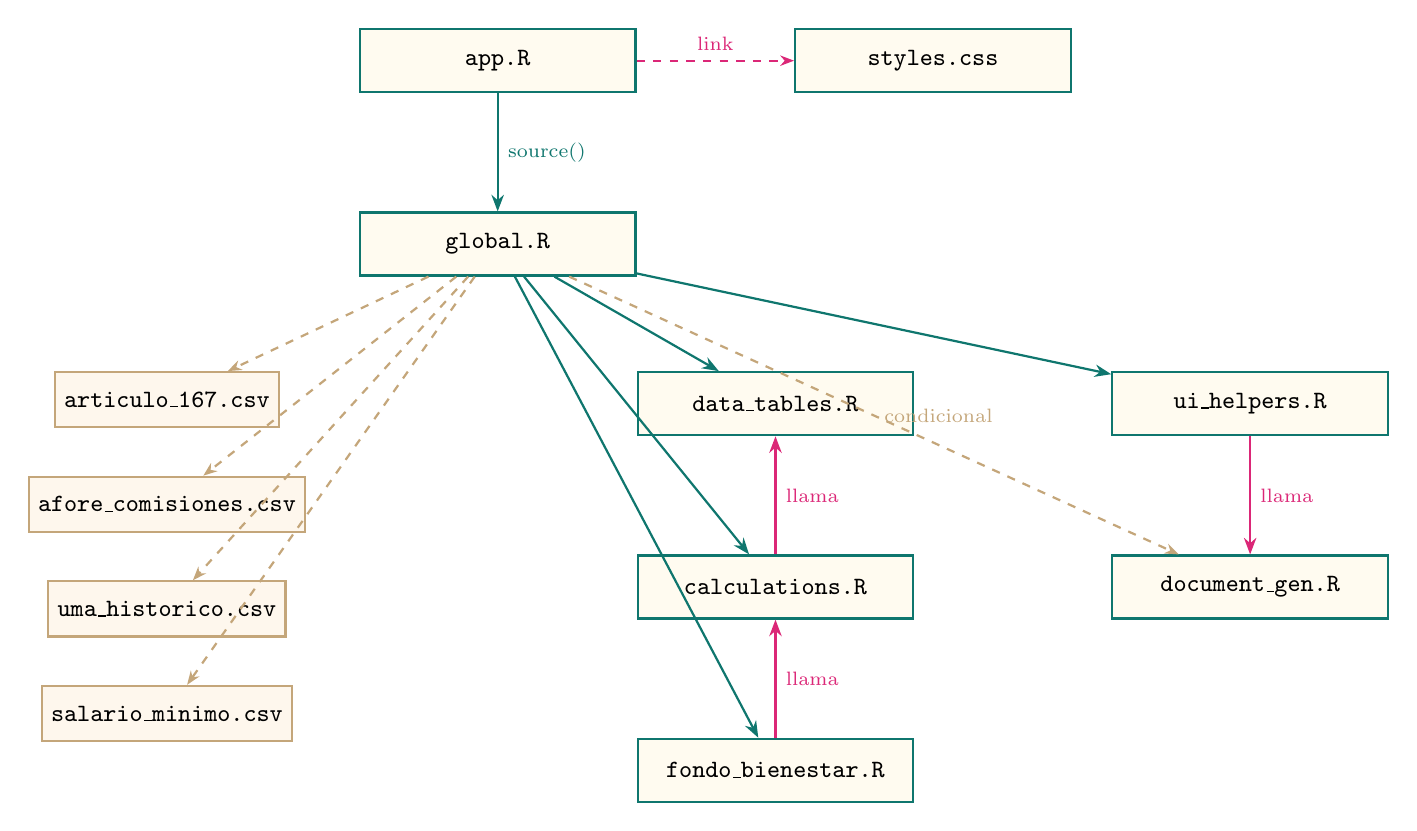
\begin{tikzpicture}[
  node distance=1.5cm and 2.5cm,
  file/.style={rectangle, draw=teal, fill=surface, thick, minimum width=3.5cm, minimum height=0.8cm, font=\small\ttfamily},
  data/.style={rectangle, draw=goldmuted, fill=bodybg, thick, minimum width=2.5cm, minimum height=0.7cm, font=\small\ttfamily},
  arr/.style={-{Stealth[length=6pt]}, thick, teal},
  darr/.style={-{Stealth[length=5pt]}, thick, goldmuted, dashed},
]

% Nodos principales
\node[file] (app) {app.R};
\node[file, below=of app] (global) {global.R};
\node[data, below left=1.2cm and 1cm of global] (csv1) {articulo\_167.csv};
\node[data, below=0.6cm of csv1] (csv2) {afore\_comisiones.csv};
\node[data, below=0.6cm of csv2] (csv3) {uma\_historico.csv};
\node[data, below=0.6cm of csv3] (csv4) {salario\_minimo.csv};
\node[file, below right=1.2cm and 0cm of global] (dt) {data\_tables.R};
\node[file, below=of dt] (calc) {calculations.R};
\node[file, below=of calc] (fondo) {fondo\_bienestar.R};
\node[file, right=2.5cm of dt] (ui) {ui\_helpers.R};
\node[file, below=of ui] (docgen) {document\_gen.R};
\node[file, right=2cm of app] (css) {styles.css};

% Flechas de source()
\draw[arr] (app) -- node[right, font=\scriptsize] {source()} (global);
\draw[arr] (global) -- (dt);
\draw[arr] (global) -- (calc);
\draw[arr] (global) -- (fondo);
\draw[arr] (global) -- (ui);
\draw[darr] (global) -- node[right, font=\scriptsize] {condicional} (docgen);

% Flechas de datos
\draw[darr] (global) -- (csv1);
\draw[darr] (global) -- (csv2);
\draw[darr] (global) -- (csv3);
\draw[darr] (global) -- (csv4);

% Dependencias entre modulos
\draw[arr, magenta] (calc) -- node[right, font=\scriptsize\color{magenta}] {llama} (dt);
\draw[arr, magenta] (fondo) -- node[right, font=\scriptsize\color{magenta}] {llama} (calc);
\draw[arr, magenta] (ui.south) -- node[right, font=\scriptsize\color{magenta}] {llama} (docgen);

% CSS
\draw[darr, magenta] (app) -- node[above, font=\scriptsize] {link} (css);

\end{tikzpicture}
\end{center}

\subsection{Patron de Doble Carga de Librerias}
\label{sec:doblecarga}

\begin{patronbox}
\textbf{Patron: Dual Library Loading.} Las librerias se cargan en \texttt{global.R}
(lineas 17--22) Y tambien se referencian con namespace en \texttt{app.R}
(por ejemplo \texttt{plotly::plotlyOutput}). Esto es necesario porque la definicion
de UI en Shiny se evalua antes de que \texttt{server()} se ejecute, y expresiones
como \texttt{plotlyOutput()} necesitan que el paquete \texttt{plotly} este disponible
en tiempo de evaluacion de UI.
\end{patronbox}

\begin{codigobox}
\texttt{global.R} linea 20: \texttt{library(plotly)} --- carga el paquete.\\
\texttt{app.R} dentro de UI: \texttt{plotly::plotlyOutput("pension\_chart")} --- referencia
explicita con namespace para evitar ambiguedad.\\
Si omites el \texttt{library()} en \texttt{global.R}, la UI falla al renderizar porque
\texttt{plotlyOutput} no existe aun cuando Shiny evalua la definicion de UI.
\end{codigobox}


\section{Constantes y Valores Regulatorios}
\label{sec:constantes}

\begin{intuicionbox}
Todas las constantes regulatorias viven en un solo lugar: \texttt{global.R} lineas
44--74. Para actualizar el simulador al ano 2026, solo necesitas cambiar $\sim$5
valores en este bloque. Los umbrales del Fondo Bienestar tienen su propia funcion
\texttt{get\_umbral\_fondo\_bienestar()} con valores historicos hardcodeados.
\end{intuicionbox}

\begin{table}[h]
\centering
\caption{Constantes regulatorias definidas en \texttt{global.R}}
\label{tab:constantes}
\begin{tabular}{llll}
\toprule
\textbf{Variable} & \textbf{Valor} & \textbf{Linea} & \textbf{Fuente} \\
\midrule
\texttt{ANIO\_ACTUAL} & 2025 & 45 & --- \\
\texttt{UMA\_DIARIA\_2025} & 113.14 & 48 & INEGI/DOF \\
\texttt{UMA\_MENSUAL\_2025} & 3,439.46 & 49 & Calculado \\
\texttt{SM\_DIARIO\_2025} & 278.80 & 52 & CONASAMI \\
\texttt{SM\_MENSUAL\_2025} & 8,474.52 & 53 & Calculado \\
\texttt{UMBRAL\_FONDO\_2025} & 17,364 & 56 & DOF/IMSS \\
\texttt{TOPE\_SBC\_DIARIO} & 2,828.50 & 59 & 25 $\times$ UMA \\
\texttt{RENDIMIENTO\_BASE} & 0.04 (4\%) & 63 & --- \\
\texttt{FACTORES\_CESANTIA} & 0.75--1.00 & 67--74 & LSS Art. 167 \\
\bottomrule
\end{tabular}
\end{table}


% =============================================================================
\chapter{Capa de Datos}
\label{ch:datos}
% =============================================================================

\section{Archivos CSV}
\label{sec:csv}

\begin{patronbox}
\textbf{Patron: Static Lookup Tables.} Los datos regulatorios se almacenan como
archivos CSV planos, cargados una sola vez al arranque via \texttt{read.csv()} con
superasignacion \texttt{<<-}. No hay base de datos, no hay API --- todo es
lectura en memoria. Esto es apropiado porque los datos regulatorios cambian
como maximo una vez al ano.
\end{patronbox}

\begin{intuicionbox}
Los 4 CSV son ``tablas de consulta'' (lookup tables). El flujo es:
\textbf{usuario ingresa salario} $\rightarrow$ se divide entre salario minimo
$\rightarrow$ se busca en \texttt{articulo\_167\_tabla.csv} $\rightarrow$ se obtiene
cuantia basica. Es un patron tipico de datos actuariales donde las formulas
dependen de rangos discretos definidos por ley.
\end{intuicionbox}

\begin{codigobox}
Archivos de datos y sus estructuras:
\begin{itemize}[nosep]
\item \texttt{data/articulo\_167\_tabla.csv}: 24 filas, columnas \texttt{grupo\_min},
      \texttt{grupo\_max}, \texttt{cuantia\_basica}, \texttt{incremento\_anual}.
      Leido en \texttt{global.R:29}.
\item \texttt{data/afore\_comisiones.csv}: 11 filas (una por AFORE), columnas
      \texttt{afore}, \texttt{comision\_2024}, \texttt{comision\_2025}, \texttt{irn\_2024}.
      Leido en \texttt{global.R:38}.
\item \texttt{data/uma\_historico.csv}: 10 filas (2016--2025), columnas \texttt{anio},
      \texttt{uma\_diaria}. Leido en \texttt{global.R:32}.
\item \texttt{data/salario\_minimo.csv}: 10 filas (2016--2025), columnas \texttt{anio},
      \texttt{sm\_diario}. Leido en \texttt{global.R:35}.
\end{itemize}
\end{codigobox}


\section{Funciones de Acceso a Datos}
\label{sec:acceso_datos}

El archivo \texttt{R/data\_tables.R} (244 lineas) provee la capa de abstraccion
sobre los datos crudos. Contiene 8 funciones publicas.

\subsection{lookup\_articulo\_167}

\begin{patronbox}
\textbf{Patron: Range Lookup.} A diferencia de un lookup por clave exacta, esta
funcion busca en \emph{rangos}: el grupo salarial debe caer entre \texttt{grupo\_min}
y \texttt{grupo\_max} de alguna fila. Si excede el maximo, usa la ultima fila;
si es menor al minimo, usa la primera. Es un patron defensivo que garantiza
que siempre se retorna un valor.
\end{patronbox}

\begin{intuicionbox}
El articulo 167 de la LSS define 24 grupos salariales. Cada grupo tiene un
``porcentaje base'' (cuantia basica) y un ``incremento por ano extra'' (incremento anual).
Un trabajador que gana 3 veces el salario minimo cae en un grupo diferente que uno
que gana 6 veces. La tabla es fija por ley --- no cambia con inflacion.
\end{intuicionbox}

\begin{codigobox}
\texttt{R/data\_tables.R} lineas 12--30:
\begin{lstlisting}[caption={lookup\_articulo\_167}]
lookup_articulo_167 <- function(grupo_salarial, tabla = articulo_167_tabla) {
  idx <- which(grupo_salarial >= tabla$grupo_min & grupo_salarial <= tabla$grupo_max)
  if (length(idx) == 0) {
    if (grupo_salarial > max(tabla$grupo_max)) {
      idx <- nrow(tabla)       # Tope superior
    } else {
      idx <- 1                 # Piso inferior
    }
  }
  return(list(
    cuantia_basica = tabla$cuantia_basica[idx],
    incremento_anual = tabla$incremento_anual[idx]
  ))
}
\end{lstlisting}
\end{codigobox}


\subsection{get\_esperanza\_vida}

\begin{patronbox}
\textbf{Patron: Interpolation with Boundary Clamping.} Para edades que no
aparecen exactamente en la tabla (como 72 o 77 anos), la funcion interpola
linealmente entre los puntos conocidos. Para edades fuera de rango, aplica
extrapolacion con limites: por debajo del minimo, suma anos directamente;
por encima del maximo, decrementa con un piso de 2 anos.
\end{patronbox}

\begin{intuicionbox}
Las tablas de mortalidad CONAPO definen puntos a edades clave (60, 65, 70, 75, 80,
85, 90). Si el usuario tiene 73 anos, necesitamos un valor entre los puntos
70 y 75. La interpolacion lineal es una simplificacion educativa --- las tablas
actuariales reales usan funciones de Gompertz-Makeham.
Mujeres viven $\sim$5 anos mas que hombres en la tabla, lo que significa menores
pensiones mensuales bajo retiro programado (mismo saldo, mas meses de vida).
\end{intuicionbox}

\begin{codigobox}
\texttt{R/data\_tables.R} lineas 89--143. Estructura interna:
\begin{lstlisting}[caption={Tablas de mortalidad con interpolacion}]
get_esperanza_vida <- function(edad, genero = "M") {
  # Validacion de NULLs (lineas 94-99)
  if (genero == "F") {
    base <- c("60"=24.5, "65"=20.0, "70"=15.9, "75"=12.5, "80"=9.5, ...)
  } else {
    base <- c("60"=21.0, "65"=17.0, "70"=13.4, "75"=10.5, "80"=8.0, ...)
  }
  # Lookup exacto (lineas 117-120)
  if (edad_str %in% names(base)) return(base[edad_str])
  # Interpolacion lineal (lineas 133-142)
  prop <- (edad - edades[idx_inf]) / (edades[idx_sup] - edades[idx_inf])
  return(valores[idx_inf] + prop * (valores[idx_sup] - valores[idx_inf]))
}
\end{lstlisting}
\end{codigobox}


\subsection{Funciones de Validacion}

\begin{patronbox}
\textbf{Patron: Structured Validation Response.} Las funciones de validacion
retornan listas con estructura fija: \texttt{\{valido, errores, advertencias\}}
para \texttt{validar\_entrada()}, y \texttt{\{is\_consistent, message\}} para
\texttt{validar\_consistencia\_fechas()}. Esto permite al server de Shiny
procesar errores y warnings por separado.
\end{patronbox}

\begin{codigobox}
Funciones de validacion en \texttt{R/data\_tables.R}:
\begin{itemize}[nosep]
\item \texttt{validar\_entrada(edad, semanas, sbc, fecha)} --- lineas 155--203.
      Valida: edad 18--90, semanas $\geq$ 0 (warn $>$ 3000), SBC $\geq$ 0,
      consistencia edad-semanas ($\text{semanas} \leq (\text{edad}-18) \times 52$),
      tope de cotizacion (25 UMA).
\item \texttt{determinar\_regimen(fecha)} --- lineas 208--222.
      Retorna \texttt{"ley73"} si fecha $<$ 1997-07-01, \texttt{"ley97"} si no.
      Convierte string a Date si necesario.
\item \texttt{validar\_consistencia\_fechas(nac, inicio)} --- lineas 228--244.
      Calcula edad de inicio de cotizacion; warn si $<$ 15 o $>$ 35.
\end{itemize}
\end{codigobox}

\subsection{Tabla Completa de Funciones de Datos}

\begin{table}[h]
\centering
\caption{Inventario de funciones en \texttt{R/data\_tables.R}}
\label{tab:data_functions}
\begin{tabularx}{\textwidth}{lclX}
\toprule
\textbf{Funcion} & \textbf{Linea} & \textbf{Retorna} & \textbf{Proposito} \\
\midrule
\texttt{lookup\_articulo\_167} & 12 & list & Busqueda por rango en tabla Art. 167 \\
\texttt{get\_afore\_names} & 38 & character & Nombres de 11 AFOREs \\
\texttt{get\_afore\_comision} & 46 & numeric & Comision con fallback a promedio \\
\texttt{get\_afore\_irn} & 63 & numeric & IRN con fallback a promedio \\
\texttt{get\_all\_afores} & 73 & data.frame & Datos completos de AFOREs \\
\texttt{get\_esperanza\_vida} & 89 & numeric & Esperanza de vida interpolada \\
\texttt{validar\_entrada} & 155 & list & Validacion de inputs del usuario \\
\texttt{determinar\_regimen} & 208 & character & Deteccion de regimen por fecha \\
\texttt{validar\_consistencia\_fechas} & 228 & list & Validacion cruzada de fechas \\
\bottomrule
\end{tabularx}
\end{table}


% =============================================================================
\chapter{Motor de Calculos Actuariales}
\label{ch:calculos}
% =============================================================================

El archivo \texttt{R/calculations.R} (671 lineas) contiene las 8 funciones que
implementan las formulas actuariales del IMSS. Este es el corazon matematico
del simulador.

\section{Ley 73: Pension Definida}
\label{sec:ley73}

\subsection{calculate\_ley73\_pension}

\begin{patronbox}
\textbf{Patron: Sequential Pipeline with Early Returns.} La funcion implementa
una cadena de 8 pasos secuenciales, con dos salidas tempranas (early returns) para
elegibilidad: semanas $<$ 500 y edad $<$ 60. Cada paso depende del anterior, y el
resultado final es una lista comprehensiva que incluye tanto el valor final como
todos los valores intermedios (para transparencia en la UI).
\end{patronbox}

\begin{intuicionbox}
La formula de Ley 73 es una cadena multiplicativa:
$$\text{pension} = \text{SBC} \times \underbrace{(\text{cuantia} + n \times \text{incremento})}_{\text{de Art. 167}} \times \underbrace{\text{factor\_edad}}_{\text{0.75--1.00}}$$
Luego se aplica un piso: la pension nunca es menor a 1 salario minimo mensual.
El factor de edad es lo que penaliza retirarse antes de los 65: a los 60 pierdes 25\%
de tu pension. Por eso el slider de edad de retiro tiene tanto impacto.
\end{intuicionbox}

\begin{codigobox}
\texttt{R/calculations.R} lineas 21--103. Los 8 pasos:
\begin{lstlisting}[caption={Cadena de Ley 73}]
calculate_ley73_pension <- function(sbc_promedio_diario, semanas, edad,
                                     sm_vigente = SM_DIARIO_2025, tipo_pension = "vejez") {
  # Early returns: semanas < 500 (linea 28), edad < 60 (linea 36)
  if (semanas < 500) return(list(pension_mensual=0, elegible=FALSE, ...))
  if (edad < 60) return(list(pension_mensual=0, elegible=FALSE, ...))

  # Paso 1: Grupo salarial (linea 45)
  grupo_salarial <- sbc_promedio_diario / sm_vigente

  # Paso 2: Busqueda Art. 167 (linea 48)
  tabla_lookup <- lookup_articulo_167(grupo_salarial)

  # Paso 3: Incrementos (linea 53)
  n_incrementos <- max(0, floor((semanas - 500) / 52))

  # Paso 4: Porcentaje total con tope 100% (linea 57)
  porcentaje_total <- min(cuantia_basica + total_incrementos, 1.0)

  # Paso 5: Factor de edad/cesantia (lineas 60-67)
  factor_edad <- if (edad >= 65) 1.0 else FACTORES_CESANTIA[as.character(edad)]

  # Paso 6: Pension diaria -> mensual (lineas 72-75)
  DIAS_POR_MES <- 30.4375  # 365.25/12, estandar actuarial
  pension_mensual <- sbc_promedio_diario * porcentaje_total * factor_edad * DIAS_POR_MES

  # Paso 7: Pension minima (lineas 78-79)
  pension_final <- max(pension_mensual, sm_vigente * DIAS_POR_MES)

  # Paso 8: Return comprehensivo (lineas 85-102)
}
\end{lstlisting}
\textbf{Nota critica}: Se usa 30.4375 dias/mes (no 30). La diferencia de 1.44\%
se acumula a lo largo de decadas y afecta la precision del calculo.
\end{codigobox}


\subsection{Diagrama de la Cadena Ley 73}

\begin{center}
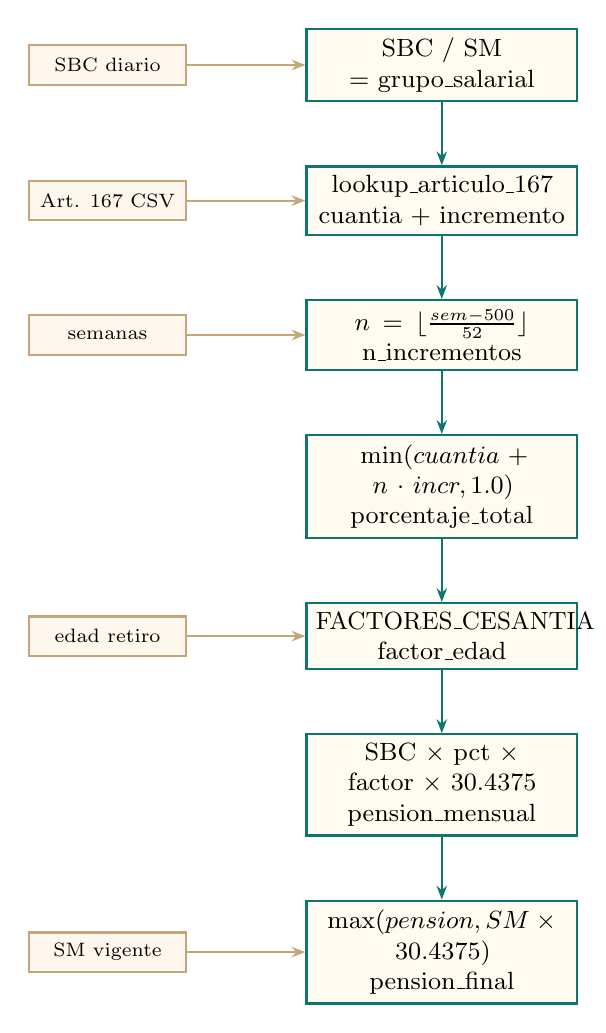
\begin{tikzpicture}[
  calcstep/.style={rectangle, draw=teal, fill=surface, thick, minimum width=3cm, minimum height=0.7cm, font=\small, text width=3.2cm, align=center},
  input/.style={rectangle, draw=goldmuted, fill=bodybg, thick, minimum width=2cm, minimum height=0.5cm, font=\scriptsize},
  arr/.style={-{Stealth[length=5pt]}, thick, teal},
  note/.style={font=\scriptsize\color{goldmuted}, text width=2.5cm, align=center},
]

\node[calcstep] (s1) {SBC / SM\\= grupo\_salarial};
\node[calcstep, below=0.8cm of s1] (s2) {lookup\_articulo\_167\\cuantia + incremento};
\node[calcstep, below=0.8cm of s2] (s3) {$n = \lfloor\frac{sem - 500}{52}\rfloor$\\n\_incrementos};
\node[calcstep, below=0.8cm of s3] (s4) {$\min(cuantia + n \cdot incr, 1.0)$\\porcentaje\_total};
\node[calcstep, below=0.8cm of s4] (s5) {FACTORES\_CESANTIA\\factor\_edad};
\node[calcstep, below=0.8cm of s5] (s6) {SBC $\times$ pct $\times$ factor $\times$ 30.4375\\pension\_mensual};
\node[calcstep, below=0.8cm of s6] (s7) {$\max(pension, SM \times 30.4375)$\\pension\_final};

% Inputs laterales
\node[input, left=1.5cm of s1] (isbc) {SBC diario};
\node[input, left=1.5cm of s2] (iart) {Art. 167 CSV};
\node[input, left=1.5cm of s3] (isem) {semanas};
\node[input, left=1.5cm of s5] (iedad) {edad retiro};
\node[input, left=1.5cm of s7] (ism) {SM vigente};

\draw[arr] (s1) -- (s2);
\draw[arr] (s2) -- (s3);
\draw[arr] (s3) -- (s4);
\draw[arr] (s4) -- (s5);
\draw[arr] (s5) -- (s6);
\draw[arr] (s6) -- (s7);

\draw[arr, goldmuted] (isbc) -- (s1);
\draw[arr, goldmuted] (iart) -- (s2);
\draw[arr, goldmuted] (isem) -- (s3);
\draw[arr, goldmuted] (iedad) -- (s5);
\draw[arr, goldmuted] (ism) -- (s7);

\end{tikzpicture}
\end{center}


\section{Ley 97: Cuenta Individual AFORE}
\label{sec:ley97}

\subsection{project\_afore\_balance}

\begin{patronbox}
\textbf{Patron: Closed-Form with Optional Simulation.} La funcion calcula el saldo
futuro usando formulas cerradas (valor futuro de lump sum + anualidad), pero
opcionalmente puede generar una trayectoria ano-por-ano usando un loop. La
trayectoria se usa para la grafica de Plotly en Step 4; el valor cerrado es mas
rapido para sensibilidad.
\end{patronbox}

\begin{intuicionbox}
El saldo futuro tiene dos componentes: (1) lo que ya tienes crece con interes
compuesto: $FV_{saldo} = S_0 \times (1+r)^n$, y (2) lo que aportas cada mes crece
como anualidad: $FV_{aport} = A \times \frac{(1+r_m)^{12n} - 1}{r_m}$.
La comision se resta del rendimiento: $r_{neto} = r_{real} - comision$.
Es una simplificacion; en realidad la comision se cobra sobre el saldo, no se resta
del rendimiento. Pero para fines educativos la diferencia es menor.
\end{intuicionbox}

\begin{codigobox}
\texttt{R/calculations.R} lineas 118--181:
\begin{lstlisting}[caption={Proyeccion AFORE con formula cerrada}]
project_afore_balance <- function(saldo_actual, aportacion_mensual,
                                   anios_al_retiro, rendimiento_real_anual = 0.04,
                                   comision_anual = 0.0053, incluir_trayectoria = FALSE) {
  r_neto <- rendimiento_real_anual - comision_anual    # linea 126
  r_mensual <- (1 + r_neto)^(1/12) - 1                # linea 129
  fv_actual <- saldo_actual * (1 + r_neto)^anios_al_retiro  # linea 133
  # Caso especial: rendimiento cero (linea 136)
  if (abs(r_mensual) < 1e-10) {
    fv_aportaciones <- aportacion_mensual * meses
  } else {
    fv_aportaciones <- aportacion_mensual * ((1+r_mensual)^meses - 1) / r_mensual
  }
  saldo_final <- fv_actual + fv_aportaciones           # linea 143
  # Trayectoria opcional (lineas 147-165): loop anual con compounding mensual
}
\end{lstlisting}
\end{codigobox}


\subsection{calculate\_aportacion\_obligatoria}

\begin{patronbox}
\textbf{Patron: Year-Indexed Rate Table.} La reforma 2020 establece un incremento
gradual de la tasa patronal de 6.20\% (2023) a 12.00\% (2030). La funcion usa un
vector nombrado para hacer lookup por ano, con fallback a 2025 si el ano no existe.
\end{patronbox}

\begin{codigobox}
\texttt{R/calculations.R} lineas 188--235:
\begin{lstlisting}[caption={Tasas de aportacion con reforma 2020}]
calculate_aportacion_obligatoria <- function(salario_mensual, anio = 2025) {
  tasas_patron <- c(
    "2023"=0.0620, "2024"=0.0690, "2025"=0.0775, "2026"=0.0860,
    "2027"=0.0945, "2028"=0.1030, "2029"=0.1115, "2030"=0.1200)
  tasa_trabajador <- 0.01125     # Fijo
  tasa_gobierno <- 0.00225       # Aproximado
  tasa_total <- tasa_patron + tasa_trabajador + tasa_gobierno
  salario_cotizable <- min(salario_mensual, TOPE_SBC_DIARIO * 30)
  aportacion <- salario_cotizable * tasa_total
}
\end{lstlisting}
\textbf{Simplificacion conocida}: El codigo usa la tasa 2025 para todos los anos
de proyeccion. La reforma per-year no se aplica aun.
\end{codigobox}


\subsection{calculate\_retiro\_programado}

\begin{patronbox}
\textbf{Patron: Floor Guarantee.} La pension por retiro programado es simplemente
$\text{saldo} / (\text{esperanza\_vida} \times 12)$, pero con un piso (floor): la
pension minima garantizada de 2.5 UMA mensuales ($\sim$\$8,599 en 2025). Cuando
el piso se activa, enmascara diferencias por genero y edad, ya que todos reciben
lo mismo.
\end{patronbox}

\begin{codigobox}
\texttt{R/calculations.R} lineas 259--298:
\begin{lstlisting}[caption={Retiro programado con pension minima}]
calculate_retiro_programado <- function(saldo, edad, genero = "M") {
  esperanza_vida <- get_esperanza_vida(edad, genero)  # linea 262
  pension_calculada <- saldo / (esperanza_vida * 12)   # linea 269
  pension_minima <- UMA_MENSUAL_2025 * 2.5             # linea 277
  aplico_minimo <- FALSE
  if (pension_calculada < pension_minima) {
    pension_mensual <- pension_minima                   # linea 283
    aplico_minimo <- TRUE
  }
}
\end{lstlisting}
Saldo necesario para superar minimo (hombre 65): $\$8,599 \times 204 = \$1,754,124$.
\end{codigobox}


\subsection{calculate\_ley97\_pension (Pipeline Completo)}

\begin{patronbox}
\textbf{Patron: Orchestrator.} Esta funcion es un orquestador que llama a
\texttt{project\_afore\_balance()} y \texttt{calculate\_retiro\_programado()}
en secuencia, agregando la logica de elegibilidad (1,000 semanas) y
seleccion de escenario (conservador/base/optimista).
\end{patronbox}

\begin{codigobox}
\texttt{R/calculations.R} lineas 313--391. Pipeline:
\begin{enumerate}[nosep]
\item Validar semanas al retiro $\geq$ 1,000 (lineas 324--334)
\item Seleccionar rendimiento por escenario (lineas 337--342)
\item Obtener comision de AFORE (linea 345)
\item Calcular aportacion obligatoria (lineas 348--349)
\item Proyectar saldo: \texttt{project\_afore\_balance()} (lineas 352--359)
\item Calcular pension: \texttt{calculate\_retiro\_programado()} (lineas 362--366)
\item Calcular tasa de reemplazo (linea 369)
\item Return comprehensivo con 18 campos (lineas 371--391)
\end{enumerate}
\end{codigobox}


\subsection{Diagrama del Pipeline Ley 97}

\begin{center}
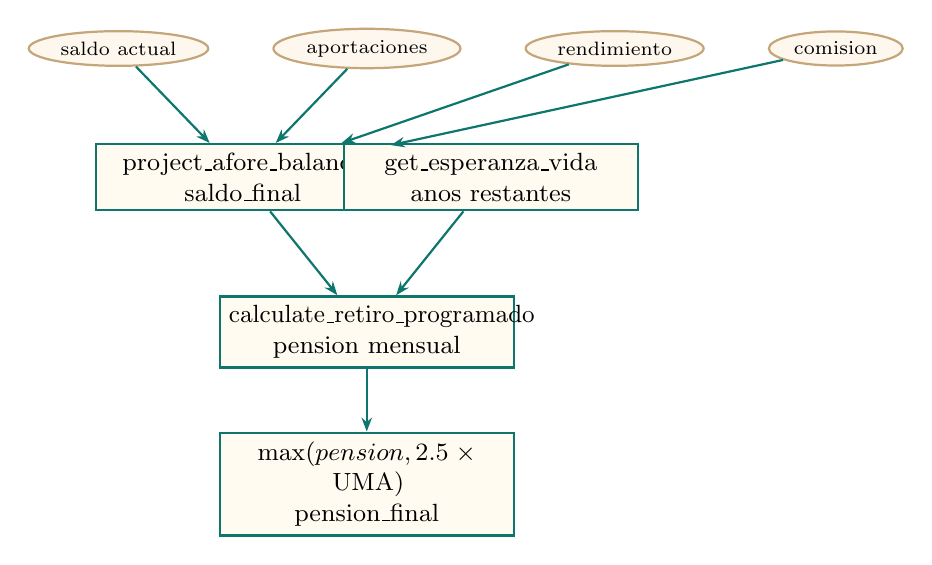
\begin{tikzpicture}[
  calcstep/.style={rectangle, draw=teal, fill=surface, thick, minimum width=3.5cm, minimum height=0.7cm, font=\small, text width=3.5cm, align=center},
  input/.style={ellipse, draw=goldmuted, fill=bodybg, thick, font=\scriptsize, inner sep=2pt},
  arr/.style={-{Stealth[length=5pt]}, thick, teal},
]

\node[input] (saldo) {saldo actual};
\node[input, right=0.8cm of saldo] (aport) {aportaciones};
\node[input, right=0.8cm of aport] (rend) {rendimiento};
\node[input, right=0.8cm of rend] (com) {comision};

\node[calcstep, below=1.2cm of $(saldo)!0.5!(aport)$] (proj) {project\_afore\_balance\\saldo\_final};
\node[calcstep, below=1.2cm of $(aport)!0.5!(rend)$] (vida) {get\_esperanza\_vida\\anos restantes};
\node[calcstep, below=1.5cm of $(proj)!0.5!(vida)$] (ret) {calculate\_retiro\_programado\\pension mensual};
\node[calcstep, below=0.8cm of ret] (min) {$\max(pension, 2.5 \times \text{UMA})$\\pension\_final};

\draw[arr] (saldo) -- (proj);
\draw[arr] (aport) -- (proj);
\draw[arr] (rend) -- (proj);
\draw[arr] (com) -- (proj);
\draw[arr] (proj) -- (ret);
\draw[arr] (vida) -- (ret);
\draw[arr] (ret) -- (min);

\end{tikzpicture}
\end{center}


\section{Modalidad 40}
\label{sec:m40}

\begin{patronbox}
\textbf{Patron: What-If Analysis.} \texttt{calculate\_modalidad\_40()} recibe la
pension actual como input y recalcula con parametros mejorados. Es un patron de
analisis ``que pasaria si'': dado que ya calculaste tu pension base, que pasa si
cotizas voluntariamente con un SBC mas alto?
\end{patronbox}

\begin{codigobox}
\texttt{R/calculations.R} lineas 412--487. Logica clave:
\begin{lstlisting}[caption={Modalidad 40 con promedio ponderado}]
# Cuota mensual M40: 10.075% del SBC elegido (lineas 425-426)
cuota_mensual_m40 <- sbc_m40_real * 30 * 0.10075

# Nuevo SBC promedio ponderado (lineas 433-441)
if (semanas_m40 >= 250) {
  nuevo_sbc_promedio <- sbc_m40_real  # M40 cubre todo el promedio
} else {
  nuevo_sbc_promedio <- (sbc_m40 * semanas_nuevas + sbc_actual * semanas_viejas) / 250
}

# Recalcular pension Ley 73 con nuevos parametros (lineas 445-450)
nueva_pension <- calculate_ley73_pension(nuevo_sbc_promedio, semanas_totales, edad)

# ROI: meses para recuperar inversion (lineas 460-464)
meses_recuperacion <- ceiling(costo_total_m40 / incremento_pension)
\end{lstlisting}
\end{codigobox}


\section{Comparacion de AFOREs}

\begin{codigobox}
\texttt{R/calculations.R} lineas 624--671. \texttt{compare\_afores()} itera sobre las
11 AFOREs, proyectando saldo con \texttt{project\_afore\_balance()} usando el IRN
de cada una como proxy de rendimiento. Retorna un \texttt{data.frame} ordenado
por saldo final, con la diferencia vs la AFORE actual del usuario.
\end{codigobox}


\section{Tabla Completa de Funciones del Motor}

\begin{table}[h]
\centering
\caption{Inventario de funciones en \texttt{R/calculations.R}}
\label{tab:calc_functions}
\begin{tabularx}{\textwidth}{lclX}
\toprule
\textbf{Funcion} & \textbf{Linea} & \textbf{Params} & \textbf{Proposito} \\
\midrule
\texttt{calculate\_ley73\_pension} & 21 & 5 & Cadena de 8 pasos Ley 73 \\
\texttt{project\_afore\_balance} & 118 & 6 & Proyeccion FV con trayectoria \\
\texttt{calculate\_aportacion\_obligatoria} & 188 & 2 & Tasas de contribucion por ano \\
\texttt{calculate\_retiro\_programado} & 259 & 3 & Pension con piso 2.5 UMA \\
\texttt{calculate\_ley97\_pension} & 313 & 9 & Pipeline completo Ley 97 \\
\texttt{calculate\_modalidad\_40} & 412 & 7 & Costo-beneficio M40 \\
\texttt{calculate\_all\_scenarios} & 498 & 9 & Multi-escenario comparativo \\
\texttt{compare\_afores} & 624 & 4 & Comparacion entre 11 AFOREs \\
\bottomrule
\end{tabularx}
\end{table}


% =============================================================================
\chapter{Modulo Fondo Bienestar}
\label{ch:fondo}
% =============================================================================

El archivo \texttt{R/fondo\_bienestar.R} (497 lineas) implementa la logica del
Fondo de Pensiones para el Bienestar, decretado el 01/05/2024 (DOF) y en vigor
desde el 01/07/2024.

\section{Elegibilidad}
\label{sec:elegibilidad}

\begin{patronbox}
\textbf{Patron: Checklist Validation.} \texttt{check\_fondo\_eligibility()} evalua
4 condiciones independientes y retorna un reporte estructurado con cada condicion
evaluada individualmente. Esto permite a la UI mostrar un checklist visual de
requisitos cumplidos/no cumplidos, en lugar de un simple ``si/no''.
\end{patronbox}

\begin{intuicionbox}
El Fondo es exclusivo para Ley 97 porque los trabajadores de Ley 73 ya tienen
pension definida (generalmente mejor). Los 4 filtros son: regimen correcto,
edad $\geq$ 65, semanas $\geq$ 1000, y salario $\leq$ umbral (\$17,364 en 2025).
El umbral sube cada ano: \$16,778 en 2024, \$17,364 en 2025, $\sim$\$18,050 en 2026.
\end{intuicionbox}

\begin{codigobox}
\texttt{R/fondo\_bienestar.R} lineas 25--92:
\begin{lstlisting}[caption={Checklist de elegibilidad del Fondo}]
check_fondo_eligibility <- function(regimen, edad, semanas,
                                     sbc_promedio_mensual, anio = ANIO_ACTUAL) {
  umbral <- get_umbral_fondo_bienestar(anio)
  checks <- list(
    regimen_valido    = list(cumple = (regimen == "ley97"), mensaje = ...),
    edad_minima       = list(cumple = (edad >= 65), mensaje = ...),
    semanas_minimas   = list(cumple = (semanas >= 1000), mensaje = ...),
    salario_bajo_umbral = list(cumple = (sbc_promedio_mensual <= umbral), mensaje = ...)
  )
  elegible <- all(sapply(checks, function(x) x$cumple))  # linea 72
  # Primera razon de no elegibilidad (lineas 76-83)
}
\end{lstlisting}
\end{codigobox}


\section{Calculo del Complemento}

\begin{patronbox}
\textbf{Patron: Gap-Fill Complement.} El complemento no es un monto fijo --- es la
diferencia entre el ``objetivo'' (menor entre salario y umbral) y la pension AFORE.
Matematicamente: $\text{complemento} = \max(0, \min(salario, umbral) - pension_{afore})$.
Si la pension AFORE ya supera el objetivo, el complemento es cero.
\end{patronbox}

\begin{codigobox}
\texttt{R/fondo\_bienestar.R} lineas 107--145:
\begin{lstlisting}[caption={Formula del complemento}]
calculate_fondo_complement <- function(pension_afore, sbc_promedio_mensual, elegibilidad) {
  if (!elegibilidad$elegible) return(list(complemento = 0, ...))
  pension_objetivo <- min(sbc_promedio_mensual, elegibilidad$umbral_usado) # linea 128
  complemento <- max(0, pension_objetivo - pension_afore)                  # linea 131
  pension_total <- pension_afore + complemento                             # linea 133
}
\end{lstlisting}
\end{codigobox}


\section{Orquestador de 3 Escenarios}
\label{sec:orquestador}

\begin{patronbox}
\textbf{Patron: Multi-Scenario Orchestrator.}
\texttt{calculate\_pension\_with\_fondo()} es la funcion central del modulo. Calcula
3 escenarios en secuencia y retorna una lista anidada con toda la informacion
para que la UI pueda renderizar el hero, el breakdown y las comparaciones.
\end{patronbox}

\begin{intuicionbox}
Los 3 escenarios responden a la pregunta clave del usuario:
\begin{enumerate}[nosep]
\item \textbf{Solo sistema}: ``Que pension me da el IMSS sin nada mas?''
\item \textbf{Con Fondo}: ``Y si califico para el Fondo Bienestar?''
\item \textbf{Con acciones}: ``Y si ademas ahorro voluntariamente?''
\end{enumerate}
La narrativa del simulador empuja al usuario hacia el escenario 3: las aportaciones
voluntarias son lo unico que el usuario controla directamente.
\end{intuicionbox}

\begin{codigobox}
\texttt{R/fondo\_bienestar.R} lineas 165--304. Estructura:
\begin{lstlisting}[caption={Orquestador de 3 escenarios}]
calculate_pension_with_fondo <- function(saldo_actual, salario_mensual,
    edad_actual, edad_retiro=65, semanas_actuales, genero="M",
    aportacion_voluntaria=0, afore_nombre="XXI Banorte", escenario="base") {

  # Escenario 1: Solo sistema (lineas 179-189)
  pension_solo <- calculate_ley97_pension(..., aportacion_voluntaria = 0)

  # Elegibilidad del Fondo (lineas 196-201)
  elegibilidad <- check_fondo_eligibility("ley97", edad_retiro, semanas_al_retiro, ...)

  # Escenario 2: Con Fondo (lineas 204-208)
  complemento <- calculate_fondo_complement(pension_solo$pension_mensual, ...)

  # Escenario 3: Con acciones del usuario (lineas 211-228)
  pension_acciones <- calculate_ley97_pension(..., aportacion_voluntaria = aportacion_voluntaria)
  complemento_acciones <- calculate_fondo_complement(pension_acciones$pension_mensual, ...)

  # Return: lista anidada con solo_sistema, con_fondo, con_acciones, fondo_bienestar
  # (lineas 232-303)
}
\end{lstlisting}
\end{codigobox}

\subsection{Diagrama de los 3 Escenarios}

\begin{center}
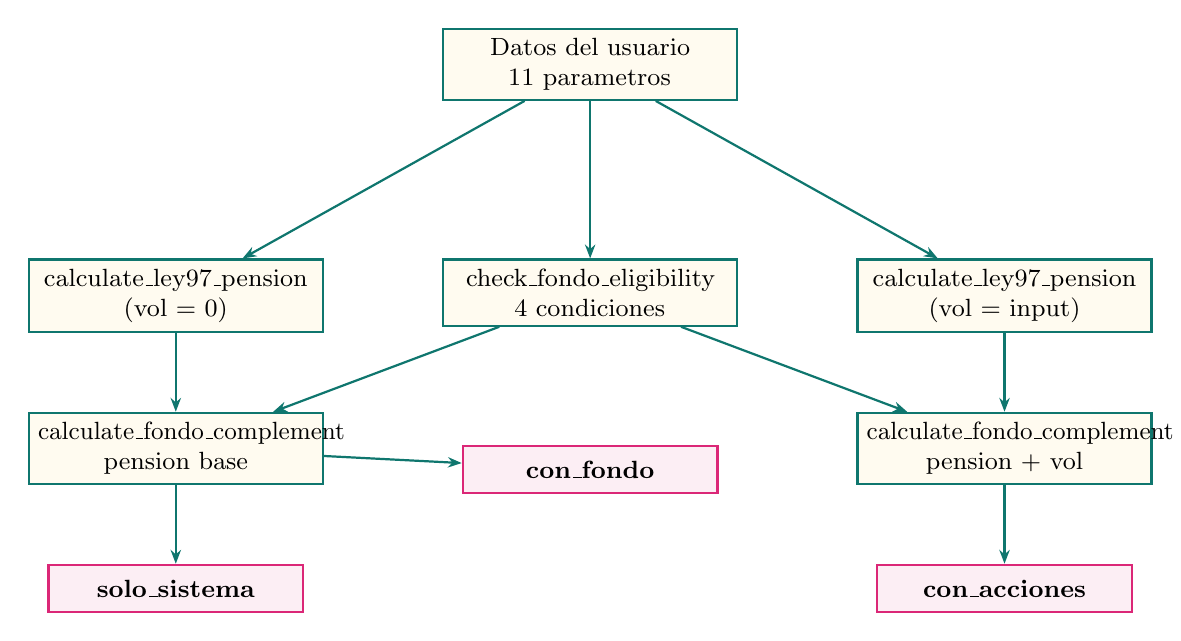
\begin{tikzpicture}[
  box/.style={rectangle, draw=teal, fill=surface, thick, minimum width=3.5cm, minimum height=0.8cm, font=\small, text width=3.5cm, align=center},
  result/.style={rectangle, draw=magenta, fill=magenta!8, thick, minimum width=3cm, minimum height=0.6cm, font=\small\bfseries, text width=3cm, align=center},
  arr/.style={-{Stealth[length=5pt]}, thick, teal},
]

% Input
\node[box] (input) {Datos del usuario\\11 parametros};

% 3 branches
\node[box, below left=2cm and 1.5cm of input] (e1) {calculate\_ley97\_pension\\(vol = 0)};
\node[box, below=2cm of input] (elig) {check\_fondo\_eligibility\\4 condiciones};
\node[box, below right=2cm and 1.5cm of input] (e3) {calculate\_ley97\_pension\\(vol = input)};

% Complements
\node[box, below=1cm of e1] (c1) {calculate\_fondo\_complement\\pension base};
\node[box, below=1cm of e3] (c3) {calculate\_fondo\_complement\\pension + vol};

% Results
\node[result, below=1cm of c1] (r1) {solo\_sistema};
\node[result, below=1.5cm of elig] (r2) {con\_fondo};
\node[result, below=1cm of c3] (r3) {con\_acciones};

\draw[arr] (input) -- (e1);
\draw[arr] (input) -- (elig);
\draw[arr] (input) -- (e3);
\draw[arr] (e1) -- (c1);
\draw[arr] (elig) -- (c1);
\draw[arr] (elig) -- (c3);
\draw[arr] (e3) -- (c3);
\draw[arr] (c1) -- (r1);
\draw[arr] (c1) -- (r2);
\draw[arr] (c3) -- (r3);

\end{tikzpicture}
\end{center}


\section{Funciones de Sensibilidad y Mensajes}

\begin{codigobox}
Funciones auxiliares en \texttt{R/fondo\_bienestar.R}:
\begin{itemize}[nosep]
\item \texttt{analyze\_voluntary\_contributions()} (lineas 315--356): Itera sobre
      un vector de aportaciones (default: 0, 500, 1000, 1500, 2000) y retorna
      un data.frame con impacto de cada una.
\item \texttt{analyze\_retirement\_age()} (lineas 363--408): Itera sobre edades
      60--70, calculando pension y elegibilidad a cada edad.
\item \texttt{generate\_personalized\_message()} (lineas 418--497): Genera mensajes
      condicionados al resultado (fondo elegible/no, tasa de reemplazo alta/media/baja,
      aportaciones voluntarias activas/inactivas).
\end{itemize}
\end{codigobox}


\section{Tabla de Funciones del Modulo Fondo}

\begin{table}[h]
\centering
\caption{Inventario de funciones en \texttt{R/fondo\_bienestar.R}}
\label{tab:fondo_functions}
\begin{tabularx}{\textwidth}{lclX}
\toprule
\textbf{Funcion} & \textbf{Linea} & \textbf{Params} & \textbf{Proposito} \\
\midrule
\texttt{check\_fondo\_eligibility} & 25 & 5 & Checklist de 4 condiciones \\
\texttt{calculate\_fondo\_complement} & 107 & 3 & Formula gap-fill \\
\texttt{calculate\_pension\_with\_fondo} & 165 & 9 & Orquestador 3 escenarios \\
\texttt{analyze\_voluntary\_contributions} & 315 & 8 & Sensibilidad aportaciones \\
\texttt{analyze\_retirement\_age} & 363 & 8 & Sensibilidad edad \\
\texttt{generate\_personalized\_message} & 418 & 1 & Mensajes personalizados \\
\bottomrule
\end{tabularx}
\end{table}


% =============================================================================
\chapter{Arquitectura UI: Componentes y Diseno}
\label{ch:ui}
% =============================================================================

\section{Sistema de Diseno CSS}
\label{sec:css}

\begin{patronbox}
\textbf{Patron: Design Tokens via CSS Custom Properties.} El archivo
\texttt{www/styles.css} define un sistema de diseno completo usando CSS custom
properties (variables) en las primeras 106 lineas. Todos los colores, sombras,
gradientes, espaciados y transiciones se referencian via variables, lo que permite
cambiar el tema entero modificando solo el bloque \texttt{:root}.
\end{patronbox}

\begin{intuicionbox}
El palette ``Tropical Vibrant'' reemplaza un diseno anterior basado en navy blue
(\texttt{\#1a365d}). La paleta actual usa teal como primario (confianza, estabilidad)
y magenta como acento (energia, accion). El fondo dorado-durazno (\texttt{\#fef7ed})
da calidez sin sacrificar legibilidad.
\end{intuicionbox}

\begin{codigobox}
\texttt{www/styles.css} lineas 9--106 (extracto de tokens):
\begin{lstlisting}[language={}, caption={Design tokens CSS}]
:root {
  --primary: #0f766e;       /* teal */
  --primary-dark: #115e59;
  --secondary: #db2777;     /* magenta */
  --secondary-light: #ec4899;
  --body-bg: #fef7ed;       /* golden-peach */
  --surface: #fffbf0;       /* card background */
  --text: #1e293b;
  --text-muted: #c4a67a;    /* golden muted */
  --border: #f0e6d6;
  --shadow-sm: 0 1px 2px rgba(15,118,110,0.06);
  --shadow-md: 0 4px 12px rgba(15,118,110,0.08);
  --transition: all 0.2s ease;
  --gradient-hero: linear-gradient(135deg, #0f766e 0%, #f97316 100%);
}
\end{lstlisting}
\end{codigobox}

\subsection{Breakpoints Responsivos}

\begin{codigobox}
Tres breakpoints en \texttt{www/styles.css}:
\begin{itemize}[nosep]
\item \texttt{@media (max-width: 992px)}: Grid 2 columnas a 1 columna,
      wizard header simplificado.
\item \texttt{@media (max-width: 768px)}: Sliders apilados verticalmente,
      fuentes reducidas.
\item \texttt{@media (max-width: 576px)}: Layout full mobile, hero compacto,
      padding reducido.
\end{itemize}
\end{codigobox}


\section{Componentes R de UI}
\label{sec:ui_components}

El archivo \texttt{R/ui\_helpers.R} (1,330 lineas) define todos los componentes de
interfaz como funciones R que retornan objetos \texttt{tagList} de Shiny.

\subsection{pension\_theme}

\begin{patronbox}
\textbf{Patron: Programmatic Theme.} En vez de definir el tema Bootstrap solo
en CSS, \texttt{pension\_theme()} usa \texttt{bslib::bs\_theme()} para configurar
Bootstrap 5 desde R, lo que permite que Shiny genere CSS coherente con el tema.
\end{patronbox}

\begin{codigobox}
\texttt{R/ui\_helpers.R} lineas 10--45:
\begin{lstlisting}[caption={Tema Bootstrap 5 programatico}]
pension_theme <- function() {
  bslib::bs_theme(
    version = 5,
    bg = "#fef7ed",
    fg = "#1e293b",
    primary = "#0f766e",
    secondary = "#db2777",
    base_font = bslib::font_google("Inter"),
    heading_font = bslib::font_google("Inter"),
    font_scale = 1.0
  )
}
\end{lstlisting}
Referencia en \texttt{app.R:20}: \texttt{theme = pension\_theme()}.
\end{codigobox}


\subsection{Landing Page Components}

\begin{codigobox}
Componentes de la pagina de aterrizaje (orden de aparicion):
\begin{itemize}[nosep]
\item \texttt{hero\_section()} (linea 53): Hero con gradiente, titulo, subtitulo,
      CTA ``Calcular mi pension'', link ``Quiero entender primero''.
\item \texttt{value\_prop\_item(icon, title, desc)} (linea 101): Card de propuesta
      de valor con icono Bootstrap.
\item \texttt{trust\_indicators()} (linea 119): Badges de confianza (``Gratis'',
      ``Sin registro'', ``100\% privado'').
\item \texttt{context\_section()} (linea 145): Seccion educativa colapsable.
\item \texttt{pension\_timeline()} (linea 197): Timeline visual de la historia
      del sistema de pensiones mexicano.
\item \texttt{comparison\_table()} (linea 244): Tabla Ley 73 vs Ley 97.
\item \texttt{control\_framework()} (linea 279): Marco verde/amarillo/rojo de
      que controla el usuario.
\end{itemize}
\end{codigobox}


\subsection{Wizard Components}

\begin{patronbox}
\textbf{Patron: Step-Based Wizard.} Los componentes del wizard
(\texttt{wizard\_header}, \texttt{wizard\_panel}) generan la estructura de un
wizard de 4 pasos. Los paneles se muestran/ocultan via \texttt{shinyjs::show/hide},
y el header se actualiza con clases CSS \texttt{.active/.completed/.upcoming}.
\end{patronbox}

\begin{codigobox}
\begin{itemize}[nosep]
\item \texttt{wizard\_header(step, total)} (linea 344): Genera indicadores de paso
      con iconos y etiquetas. Clase \texttt{.wizard-step} con modificadores.
\item \texttt{wizard\_panel(step, ...)} (linea 384): Wrapper de contenido de cada paso
      con \texttt{id = paste0("step", step, "\_panel")}.
\end{itemize}
Los 4 pasos en \texttt{app.R} UI (lineas 180--720):
\begin{enumerate}[nosep]
\item \textbf{Datos personales}: fecha nacimiento, genero, edad retiro
\item \textbf{Datos laborales}: fecha inicio cotizacion, salario, semanas
\item \textbf{AFORE}: seleccion de AFORE, saldo, aportaciones voluntarias
\item \textbf{Resultados}: hero, breakdown, sliders de sensibilidad, grafica, reportes
\end{enumerate}
\end{codigobox}


\subsection{Result Rendering}

\begin{patronbox}
\textbf{Patron: Regime-Dispatched Rendering.} El sistema usa dos funciones
separadas para renderizar resultados: \texttt{render\_results\_hero()} para Ley 97
y \texttt{render\_results\_hero\_ley73()} para Ley 73. Esto refleja que los dos
regimenes tienen estructuras de resultado fundamentalmente diferentes.
\end{patronbox}

\begin{intuicionbox}
Para Ley 97, el resultado principal es la pension AFORE con complemento del Fondo
y el impacto de aportaciones voluntarias. El hero muestra 3 escenarios apilados.
Para Ley 73, el resultado principal es la pension definida, con Modalidad 40 como
alternativa. No hay Fondo Bienestar --- es irrelevante para Ley 73.
\end{intuicionbox}

\begin{codigobox}
Funciones de renderizado de resultados en \texttt{R/ui\_helpers.R}:
\begin{itemize}[nosep]
\item \texttt{result\_card(type, title, value, subtitle)} (linea 453): Card individual
      de resultado. \texttt{type} $\in$ \{``base'', ``fondo'', ``acciones''\}.
\item \texttt{detect\_result\_scenario(resultado)} (linea 490): Clasifica el resultado
      para determinar que renderizar.
\item \texttt{render\_results\_hero(resultado)} (linea 511): Ley 97 --- hero section con
      pension principal, breakdown (AFORE vs Fondo vs Voluntarias), y tasa de reemplazo.
      228 lineas de HTML generation.
\item \texttt{render\_results\_hero\_ley73(resultado)} (linea 743): Ley 73 --- hero con
      pension definida, desglose de formula (cuantia, incrementos, factor cesantia),
      y opcion Modalidad 40. 168 lineas.
\item \texttt{encouragement\_message(resultado)} (linea 919): Mensaje motivacional
      condicionado a la tasa de reemplazo y elegibilidad del Fondo.
\end{itemize}
\end{codigobox}


\subsection{Componentes Auxiliares de UI}

\begin{codigobox}
Otros componentes en \texttt{R/ui\_helpers.R}:
\begin{itemize}[nosep]
\item \texttt{help\_tooltip(text)} (linea 994): Tooltip con icono ``?''.
\item \texttt{input\_with\_help(input, help\_text)} (linea 1007): Wrapper input + tooltip.
\item \texttt{GLOSARIO} (linea 1028): Lista nombrada con 14 terminos definidos.
\item \texttt{glossary\_panel()} (linea 1072): Accordion UI con el glosario.
\item \texttt{alert\_message(type, title, msg)} (linea 1105): Componente de alerta.
\item \texttt{technical\_panel(resultado)} (linea 1148): Accordion con detalles tecnicos
      del calculo (valores intermedios, parametros usados).
\item \texttt{replacement\_rate\_bar(tasa)} (linea 1219): Barra visual de tasa de reemplazo
      con colores condicionados (verde $>$ 70\%, amarillo 40--70\%, rojo $<$ 40\%).
\item \texttt{download\_section()} (linea 1263): Botones de descarga de reportes.
\end{itemize}
\end{codigobox}


\section{Tabla de Componentes UI}

\begin{longtable}{lclp{5.5cm}}
\caption{Inventario de funciones en \texttt{R/ui\_helpers.R}} \label{tab:ui_functions} \\
\toprule
\textbf{Funcion} & \textbf{Linea} & \textbf{Cat.} & \textbf{Proposito} \\
\midrule
\endfirsthead
\toprule
\textbf{Funcion} & \textbf{Linea} & \textbf{Cat.} & \textbf{Proposito} \\
\midrule
\endhead
\texttt{pension\_theme} & 10 & Tema & bslib Bootstrap 5 theme \\
\texttt{hero\_section} & 53 & Landing & Hero con gradiente \\
\texttt{value\_prop\_item} & 101 & Landing & Card de propuesta de valor \\
\texttt{trust\_indicators} & 119 & Landing & Badges de confianza \\
\texttt{context\_section} & 145 & Landing & Seccion educativa \\
\texttt{pension\_timeline} & 197 & Landing & Timeline historico \\
\texttt{comparison\_table} & 244 & Landing & Tabla Ley73 vs Ley97 \\
\texttt{control\_framework} & 279 & Landing & Marco verde/amarillo/rojo \\
\texttt{wizard\_header} & 344 & Wizard & Indicadores de paso \\
\texttt{wizard\_panel} & 384 & Wizard & Panel de contenido \\
\texttt{result\_card} & 453 & Results & Card de resultado \\
\texttt{detect\_result\_scenario} & 490 & Results & Clasificador de resultado \\
\texttt{render\_results\_hero} & 511 & Results & Hero Ley 97 (228 lines) \\
\texttt{render\_results\_hero\_ley73} & 743 & Results & Hero Ley 73 (168 lines) \\
\texttt{encouragement\_message} & 919 & Results & Mensaje motivacional \\
\texttt{help\_tooltip} & 994 & Form & Tooltip ``?'' \\
\texttt{input\_with\_help} & 1007 & Form & Input + tooltip wrapper \\
\texttt{GLOSARIO} & 1028 & Ref & 14 terminos definidos \\
\texttt{glossary\_panel} & 1072 & Ref & Accordion glosario \\
\texttt{alert\_message} & 1105 & Feedback & Componente de alerta \\
\texttt{technical\_panel} & 1148 & Results & Detalles tecnicos accordion \\
\texttt{replacement\_rate\_bar} & 1219 & Results & Barra tasa de reemplazo \\
\texttt{download\_section} & 1263 & Results & Botones de descarga \\
\bottomrule
\end{longtable}


% =============================================================================
\chapter{Flujo Reactivo del Servidor}
\label{ch:server}
% =============================================================================

Este capitulo mapea el grafo reactivo completo del servidor Shiny en \texttt{app.R}
(lineas 743--1,951). El servidor gestiona 8 valores reactivos, $\sim$20 observers,
y multiples outputs.

\section{Estado Reactivo}
\label{sec:estado}

\begin{patronbox}
\textbf{Patron: Centralized Reactive State.} El servidor define 8
\texttt{reactiveVal()}s que actuan como store central. A diferencia de un
\texttt{reactiveValues()} (que seria un store unico con multiples slots), se
usan \texttt{reactiveVal()}s individuales para granularidad de invalidacion:
modificar \texttt{resultados()} no invalida observers que solo dependen de
\texttt{current\_step()}.
\end{patronbox}

\begin{codigobox}
\texttt{app.R} lineas 765--784:
\begin{lstlisting}[caption={Los 8 reactiveVals del servidor}]
current_step <- reactiveVal(1)                    # Paso del wizard (1-4)
resultados <- reactiveVal(NULL)                   # Resultados actuales (con sliders)
resultados_originales <- reactiveVal(NULL)        # Baseline fijo para grafico
regimen_actual <- reactiveVal("ley97")            # Regimen detectado/override
prev_fondo_eligible <- reactiveVal(NULL)          # Tracker para cliff notification
prev_aplico_minimo <- reactiveVal(NULL)           # Tracker para pension minima
fecha_cotizacion_user_edited <- reactiveVal(FALSE)# Flag de edicion manual
regimen_override_active_val <- reactiveVal(FALSE) # Flag de override manual
\end{lstlisting}
\end{codigobox}


\section{Transiciones de Estado del Wizard}

\begin{patronbox}
\textbf{Patron: State Machine via Show/Hide.} El wizard no usa una libreria
de routing --- simplemente muestra/oculta paneles con \texttt{shinyjs::show/hide}.
El estado \texttt{current\_step()} es la ``fuente de verdad'' del paso actual.
Las transiciones estan protegidas por validacion en cada paso.
\end{patronbox}

\begin{center}
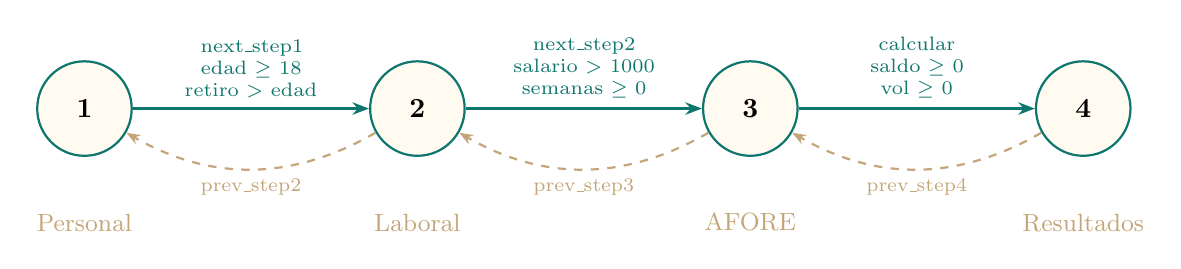
\begin{tikzpicture}[
  state/.style={circle, draw=teal, fill=surface, thick, minimum size=1.2cm, font=\bfseries},
  arr/.style={-{Stealth[length=6pt]}, thick, teal},
  back/.style={-{Stealth[length=5pt]}, thick, goldmuted, dashed, bend left=30},
  label/.style={font=\scriptsize, text width=2.5cm, align=center},
]

\node[state] (s1) {1};
\node[state, right=3cm of s1] (s2) {2};
\node[state, right=3cm of s2] (s3) {3};
\node[state, right=3cm of s3] (s4) {4};

\draw[arr] (s1) -- node[above, label] {next\_step1\\edad $\geq$ 18\\retiro $>$ edad} (s2);
\draw[arr] (s2) -- node[above, label] {next\_step2\\salario $>$ 1000\\semanas $\geq$ 0} (s3);
\draw[arr] (s3) -- node[above, label] {calcular\\saldo $\geq$ 0\\vol $\geq$ 0} (s4);

\draw[back] (s2) to node[below, font=\scriptsize] {prev\_step2} (s1);
\draw[back] (s3) to node[below, font=\scriptsize] {prev\_step3} (s2);
\draw[back] (s4) to node[below, font=\scriptsize] {prev\_step4} (s3);

% Labels debajo
\node[below=0.6cm of s1, font=\small\color{goldmuted}] {Personal};
\node[below=0.6cm of s2, font=\small\color{goldmuted}] {Laboral};
\node[below=0.6cm of s3, font=\small\color{goldmuted}] {AFORE};
\node[below=0.6cm of s4, font=\small\color{goldmuted}] {Resultados};

\end{tikzpicture}
\end{center}

\begin{codigobox}
Validaciones por paso:
\begin{itemize}[nosep]
\item \textbf{Step 1 $\to$ 2} (lineas 831--873): \texttt{fecha\_nacimiento} no NULL,
      edad $\geq$ 18, \texttt{edad\_retiro} 60--70, retiro $>$ edad actual.
\item \textbf{Step 2 $\to$ 3} (lineas 884--917): \texttt{salario\_mensual} $\geq$ 1000,
      \texttt{semanas\_cotizadas} $\geq$ 0, \texttt{fecha\_inicio\_cotizacion} valida
      y no futura.
\item \textbf{Step 3 $\to$ 4} (lineas 1046--1150): \texttt{saldo\_afore} $\geq$ 0,
      \texttt{aportacion\_voluntaria} $\geq$ 0. Dispara calculo completo.
\end{itemize}
\end{codigobox}


\section{Auto-fill y Deteccion de Regimen}
\label{sec:autofill}

\begin{patronbox}
\textbf{Patron: Cascading Defaults with Override.} La fecha de nacimiento
auto-rellena la fecha de inicio de cotizacion (nacimiento + 18 anos), que a su vez
auto-determina el regimen (Ley 73 si $<$ 1997-07-01). Ambos auto-fills tienen
flags de override: \texttt{fecha\_cotizacion\_user\_edited} y
\texttt{regimen\_override\_active\_val} previenen que ediciones manuales se
sobrescriban.
\end{patronbox}

\begin{codigobox}
Flujo de auto-fill (\texttt{app.R}):
\begin{lstlisting}[caption={Cascada fecha nacimiento -> regimen}]
# 1. Fecha nacimiento -> auto-fill fecha inicio (lineas 931-938)
observeEvent(input$fecha_nacimiento, {
  if (!fecha_cotizacion_user_edited()) {
    default_start <- input$fecha_nacimiento + as.difftime(18*365.25, units="days")
    updateDateInput(session, "fecha_inicio_cotizacion", value = default_start)
  }
})

# 2. Track de edicion manual (lineas 941-943)
observeEvent(input$fecha_inicio_cotizacion, {
  if (current_step() >= 2) fecha_cotizacion_user_edited(TRUE)
}, ignoreInit = TRUE)

# 3. Fecha inicio -> regimen automatico (lineas 949-963)
observeEvent(input$fecha_inicio_cotizacion, {
  if (!regimen_override_active_val()) {
    regimen_actual(determinar_regimen(input$fecha_inicio_cotizacion))
  }
  # Cross-validacion edad de inicio (lineas 957-962)
})

# 4. Override manual de regimen (lineas 966-977)
observeEvent(input$regimen_manual, {
  if (regimen_override_active_val()) regimen_actual(input$regimen_manual)
})
\end{lstlisting}
\end{codigobox}


\section{Calculo Principal}
\label{sec:calculo_principal}

\begin{patronbox}
\textbf{Patron: Regime Dispatch.} El \texttt{observeEvent(input\$calcular)} en
linea 1046 es el dispatcher central. Segun el regimen detectado, despacha
a \texttt{calculate\_ley73\_pension()} (con M40 opcional) o a
\texttt{calculate\_pension\_with\_fondo()} (que internamente calcula los 3 escenarios).
El resultado se almacena en \texttt{resultados()} Y en \texttt{resultados\_originales()}.
\end{patronbox}

\begin{intuicionbox}
El patron dual-store es fundamental: \texttt{resultados()} se actualiza cada vez
que un slider cambia (para actualizar la UI), pero \texttt{resultados\_originales()}
permanece fijo al valor del calculo inicial. Esto permite que la grafica de Plotly
muestre una ``linea base'' inmovil contra la cual comparar los cambios de sensibilidad.
\end{intuicionbox}

\begin{codigobox}
\texttt{app.R} lineas 1046--1150 (estructura):
\begin{lstlisting}[caption={Dispatch principal de calculo}]
observeEvent(input$calcular, {
  # Validaciones (lineas 1050-1059)
  edad_actual <- as.numeric(difftime(Sys.Date(), input$fecha_nacimiento, ...)) / 365.25

  if (regimen == "ley73") {
    # Branch Ley 73 (lineas 1068-1108)
    resultado_base <- calculate_ley73_pension(sbc_diario, semanas_al_retiro, edad_retiro)
    resultado_m40 <- calculate_modalidad_40(...)  # si elegible y anios > 0
    res <- list(regimen="ley73", pension_base=resultado_base, pension_m40=resultado_m40)
  } else {
    # Branch Ley 97 (lineas 1110-1125)
    res <- calculate_pension_with_fondo(saldo, salario, edad, ...)
    res$regimen <- "ley97"
  }

  resultados(res)                    # Mutable: actualizado por sliders
  resultados_originales(res)         # Inmutable: baseline para grafico

  # Inicializar sliders con valores actuales (lineas 1140-1143)
  # Transicion visual al paso 4 (lineas 1146-1149)
})
\end{lstlisting}
\end{codigobox}


\section{Sensibilidad con Debounce}
\label{sec:sensibilidad}

\begin{patronbox}
\textbf{Patron: Debounced Reactive Chain.} Los 5 sliders de sensibilidad pasan
por \texttt{debounce(300)} antes de alimentar al observer unificado de recalculo.
El debounce previene que cada tick del slider dispare un recalculo completo ---
solo se recalcula 300ms despues del ultimo movimiento.
\end{patronbox}

\begin{intuicionbox}
Sin debounce, mover un slider de 1000 a 2000 pesos dispararia $\sim$1000
recalculos (uno por cada peso). Con debounce de 300ms, solo se dispara 1 recalculo
al final del movimiento. Esto es critico para performance porque cada recalculo
invoca \texttt{calculate\_pension\_with\_fondo()} que a su vez llama a
\texttt{calculate\_ley97\_pension()} dos veces.
\end{intuicionbox}

\begin{codigobox}
\texttt{app.R} lineas 1174--1179 (debounce) y 1205--1306 (recalculo unificado):
\begin{lstlisting}[caption={Debounce y recalculo unificado}]
# Debounce de 300ms para cada slider (lineas 1174-1179)
vol_debounced <- reactive({ input$slider_voluntaria }) |> debounce(300)
edad_debounced <- reactive({ input$slider_edad }) |> debounce(300)
semanas_debounced <- reactive({ input$slider_semanas }) |> debounce(300)
afore_debounced <- reactive({ input$afore_comparar }) |> debounce(300)
salario_debounced <- reactive({ input$slider_salario }) |> debounce(300)

# Observer unificado (linea 1205)
observe({
  req(resultados_originales())
  res_orig <- resultados_originales()

  # Leer valores debounced con fallback %||% (lineas 1209-1213)
  vol_actual <- vol_debounced() %||% res_orig$entrada$aportacion_voluntaria %||% 0
  edad_slider <- edad_debounced() %||% res_orig$entrada$edad_retiro
  # ...

  if (res_orig$regimen == "ley97") {
    res <- calculate_pension_with_fondo(...)   # Recalculo completo
    # Cliff notifications (lineas 1231-1280)
    resultados(res)                            # Actualizar store mutable
  } else {  # ley73
    resultado_base <- calculate_ley73_pension(...)
    resultado_m40 <- calculate_modalidad_40(...)
    resultados(list(...))
  }
})
\end{lstlisting}
\end{codigobox}


\section{Impact Labels (Etiquetas de Impacto)}
\label{sec:impact_labels}

\begin{patronbox}
\textbf{Patron: Delta Display.} Para cada slider, un observer dedicado calcula
la diferencia entre el valor original (baseline) y el valor actual (con slider).
El resultado se muestra como etiqueta coloreada: verde si positivo, rojo si
negativo, gris si neutral.
\end{patronbox}

\begin{codigobox}
\texttt{app.R} lineas 1308--1638. Hay 5 observers de impact label:
\begin{itemize}[nosep]
\item \texttt{slider\_voluntaria} $\to$ \texttt{vol\_impact} (lineas 1309--1355)
\item \texttt{slider\_edad} $\to$ \texttt{age\_impact} (lineas 1358--1420)
\item \texttt{afore\_comparar} $\to$ \texttt{afore\_impact} (lineas 1424--1483)
\item \texttt{slider\_semanas} $\to$ \texttt{semanas\_impact} (lineas 1486--1575)
\item \texttt{slider\_salario} $\to$ \texttt{salario\_impact} (lineas 1579--1638)
\end{itemize}
Patron comun: obtener pension original de \texttt{resultados\_originales()},
pension actual de \texttt{resultados()}, calcular diferencia y porcentaje,
generar HTML con color condicionado.
\end{codigobox}


\section{Cliff Notifications}
\label{sec:cliff}

\begin{patronbox}
\textbf{Patron: State Transition Alerts.} El sistema detecta cuando un cambio
de slider cruza un umbral critico (por ejemplo, perder elegibilidad del Fondo o
caer en pension minima) y muestra una notificacion unica. Los
\texttt{reactiveVal}s \texttt{prev\_fondo\_eligible} y \texttt{prev\_aplico\_minimo}
rastrean el estado anterior para detectar transiciones.
\end{patronbox}

\begin{codigobox}
\texttt{app.R} lineas 1231--1280 (dentro del observer unificado):
\begin{lstlisting}[caption={Deteccion de cliff notifications}]
# Cliff: perdida de elegibilidad al Fondo (lineas 1232-1248)
prev_eligible <- isolate(prev_fondo_eligible())
new_eligible <- res$con_fondo$elegible
if (!is.null(prev_eligible) && prev_eligible != new_eligible) {
  if (!new_eligible) {
    showNotification("Con estos cambios pierdes elegibilidad...", type="warning")
  } else {
    showNotification("Con estos cambios ganas elegibilidad!", type="message")
  }
}
prev_fondo_eligible(new_eligible)

# Cliff: caida/salida de pension minima (lineas 1254-1278)
# Similar: compara prev_aplico_minimo con nuevo estado
\end{lstlisting}
\end{codigobox}


\section{Grafica Plotly}
\label{sec:plotly}

\begin{patronbox}
\textbf{Patron: Dual-Dispatch Chart.} La grafica usa dos modos completamente
diferentes segun el regimen: barras horizontales para Ley 73, y 3 trazos de linea
superpuestos para Ley 97 (trayectoria de saldo AFORE a lo largo del tiempo).
\end{patronbox}

\begin{codigobox}
\texttt{app.R} lineas 1658--1777. Estructura:
\begin{lstlisting}[caption={Grafica Plotly dual-mode}]
output$pension_chart <- plotly::renderPlotly({
  req(resultados())
  if (resultados()$regimen == "ley73") {
    # Barras horizontales: pension base vs M40 (lineas 1667-1720)
    plot_ly(type="bar", orientation="h", ...)
  } else {
    # Ley 97: 3 trazos superpuestos (lineas 1725-1770)
    # Trazo 1: baseline (dorado punteado) - de resultados_originales()
    # Trazo 2: con cambios (teal discontinuo) - de resultados()
    # Trazo 3: con aportaciones (teal solido) - de resultados() con vol > 0
    plot_ly() |>
      add_trace(trayectoria_original, line=list(dash="dot", color="#c4a67a")) |>
      add_trace(trayectoria_actual, line=list(dash="dash", color="#0f766e")) |>
      add_trace(trayectoria_acciones, line=list(color="#0f766e"))
  }
})
\end{lstlisting}
Los 3 trazos usan trayectorias de \texttt{resultados\_originales()} (baseline) y
\texttt{resultados()} (con sliders), lo que permite ver el impacto visual de cada cambio.
\end{codigobox}


\section{Diagrama del Grafo Reactivo Completo}

\begin{center}
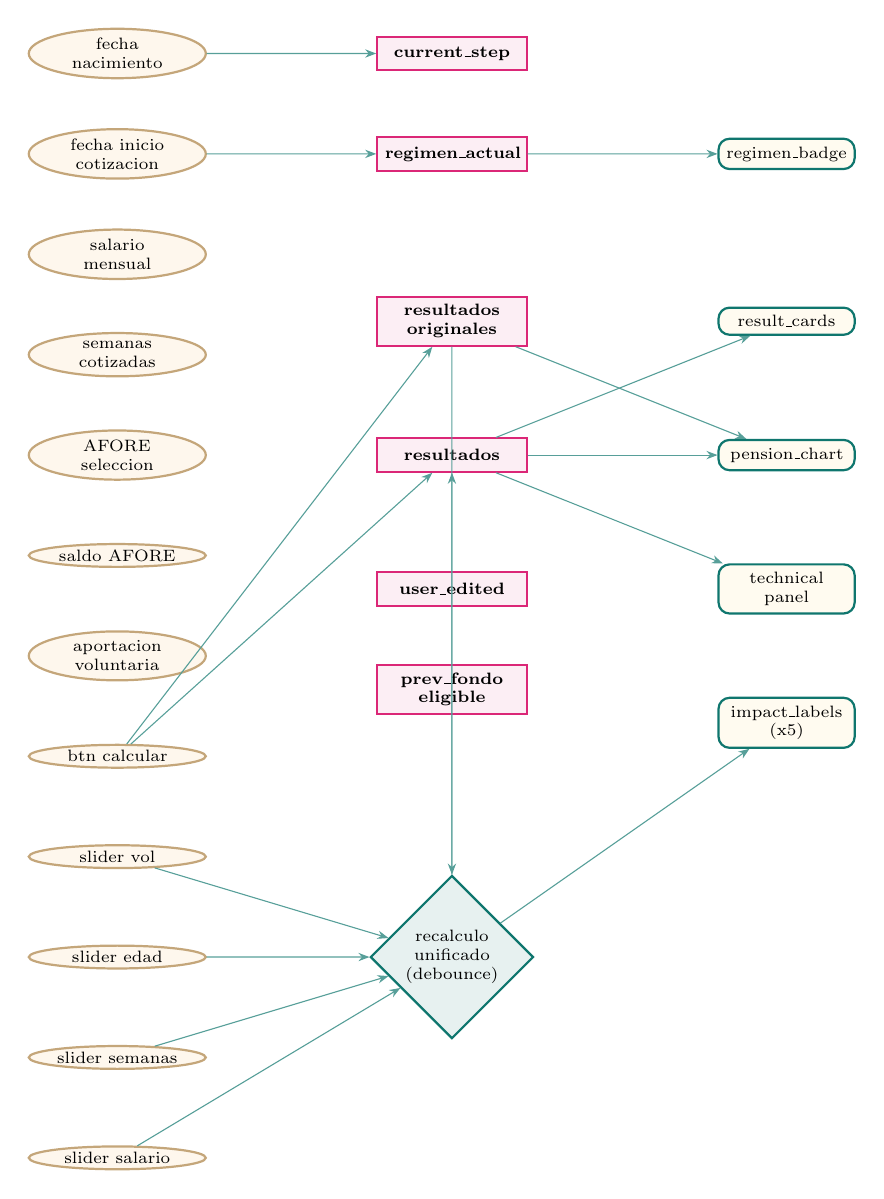
\begin{tikzpicture}[
  input/.style={ellipse, draw=goldmuted, fill=bodybg, thick, font=\scriptsize, inner sep=1pt, text width=1.8cm, align=center},
  rv/.style={rectangle, draw=magenta, fill=magenta!8, thick, font=\scriptsize\bfseries, minimum width=2cm, minimum height=0.5cm, text width=2cm, align=center},
  obs/.style={diamond, draw=teal, fill=teal!10, thick, font=\scriptsize, inner sep=1pt, text width=1.5cm, align=center},
  outputnode/.style={rectangle, draw=teal, fill=surface, thick, rounded corners, font=\scriptsize, minimum width=1.8cm, minimum height=0.4cm, text width=1.8cm, align=center},
  arr/.style={-{Stealth[length=4pt]}, thin, teal!70},
  scale=0.85, transform shape,
]

% Inputs (izquierda)
\node[input] (fnac) at (0, 8) {fecha\\ nacimiento};
\node[input] (finicio) at (0, 6.5) {fecha inicio\\cotizacion};
\node[input] (sal) at (0, 5) {salario\\mensual};
\node[input] (sem) at (0, 3.5) {semanas\\cotizadas};
\node[input] (afore) at (0, 2) {AFORE\\seleccion};
\node[input] (saldo) at (0, 0.5) {saldo AFORE};
\node[input] (vol) at (0, -1) {aportacion\\voluntaria};
\node[input] (calcbtn) at (0, -2.5) {btn calcular};

% ReactiveVals (centro)
\node[rv] (step) at (5, 8) {current\_step};
\node[rv] (regimen) at (5, 6.5) {regimen\_actual};
\node[rv] (resorig) at (5, 4) {resultados\\originales};
\node[rv] (res) at (5, 2) {resultados};
\node[rv] (usered) at (5, 0) {user\_edited};
\node[rv] (prevelig) at (5, -1.5) {prev\_fondo\\eligible};

% Sliders (debounced)
\node[input] (svol) at (0, -4) {slider vol};
\node[input] (sedad) at (0, -5.5) {slider edad};
\node[input] (ssem) at (0, -7) {slider semanas};
\node[input] (ssal) at (0, -8.5) {slider salario};

% Observer unificado
\node[obs] (recalc) at (5, -5.5) {recalculo\\unificado\\(debounce)};

% Outputs (derecha)
\node[outputnode] (rcards) at (10, 4) {result\_cards};
\node[outputnode] (badge) at (10, 6.5) {regimen\_badge};
\node[outputnode] (chart) at (10, 2) {pension\_chart};
\node[outputnode] (impacts) at (10, -2) {impact\_labels (x5)};
\node[outputnode] (tech) at (10, 0) {technical panel};

% Arrows inputs -> reactiveVals
\draw[arr] (fnac) -- (step);
\draw[arr] (finicio) -- (regimen);
\draw[arr] (calcbtn) -- (resorig);
\draw[arr] (calcbtn) -- (res);

% Arrows reactiveVals -> outputs
\draw[arr] (regimen) -- (badge);
\draw[arr] (res) -- (rcards);
\draw[arr] (res) -- (chart);
\draw[arr] (resorig) -- (chart);
\draw[arr] (res) -- (tech);

% Sliders -> recalculation
\draw[arr] (svol) -- (recalc);
\draw[arr] (sedad) -- (recalc);
\draw[arr] (ssem) -- (recalc);
\draw[arr] (ssal) -- (recalc);
\draw[arr] (recalc) -- (res);
\draw[arr] (recalc) -- (impacts);
\draw[arr] (resorig) -- (recalc);

\end{tikzpicture}
\end{center}


% =============================================================================
\chapter{Pipeline de Generacion de Documentos}
\label{ch:docgen}
% =============================================================================

El archivo \texttt{R/document\_generators.R} (1,667 lineas) implementa la generacion
de reportes HTML y PDF/RMarkdown.

\section{Arquitectura de Reportes}
\label{sec:reportes}

\begin{patronbox}
\textbf{Patron: Dual Format Generation.} Cada tipo de reporte tiene dos
implementaciones: una directa en HTML (para visualizacion rapida en navegador)
y una en RMarkdown (para compilacion a PDF via pandoc/LaTeX). La version HTML es
la preferida porque no requiere dependencias externas.
\end{patronbox}

\begin{intuicionbox}
El pipeline de reportes es: usuario clickea boton $\to$ se genera HTML en un
archivo temporal en \texttt{www/} $\to$ JavaScript abre una nueva pestana del
navegador $\to$ cuando la sesion termina, se borran los archivos temporales.
La carpeta \texttt{www/} se usa porque Shiny sirve su contenido como archivos
estaticos accesibles via URL.
\end{intuicionbox}

\begin{codigobox}
Funciones de generacion en \texttt{R/document\_generators.R}:
\begin{itemize}[nosep]
\item \texttt{get\_document\_css()} (linea 10): CSS compartido para todos los reportes.
      Usa la misma paleta Tropical Vibrant.
\item \texttt{generate\_basic\_report(resultado, output\_file)} (linea 1047): Reporte
      basico HTML --- resumen de pension, datos de entrada, resultado principal.
\item \texttt{generate\_technical\_report(resultado, output\_file)} (linea 756): Reporte
      tecnico HTML --- incluye todos los valores intermedios del calculo.
\item \texttt{generate\_methodology\_html(output\_file)} (linea 1200): Documento de
      metodologia estatico (no depende de resultado).
\item \texttt{generate\_summary\_report(resultado, output\_file)} (linea 1545): Resumen
      ejecutivo HTML.
\item \texttt{generate\_basic\_rmd(resultado, output\_file)} (linea 410): RMarkdown basico.
\item \texttt{generate\_technical\_rmd(resultado, output\_file)} (linea 523): RMarkdown tecnico.
\item \texttt{generate\_summary\_rmd(resultado, output\_file)} (linea 1444): RMarkdown resumen.
\item \texttt{generate\_methodology\_pdf(output\_file)} (linea 341): Metodologia RMarkdown/PDF.
\end{itemize}
\end{codigobox}


\section{Ciclo de Vida de Archivos Temporales}

\begin{patronbox}
\textbf{Patron: Session-Scoped Temp Files.} Los reportes se generan como archivos
temporales en el directorio \texttt{www/} del servidor. Cada archivo recibe un
nombre unico via \texttt{tempfile()}. Cuando la sesion de Shiny termina, un
callback registrado con \texttt{session\$onSessionEnded} limpia los archivos.
\end{patronbox}

\begin{codigobox}
\texttt{app.R} lineas 1868--1932 (patron de generacion y limpieza):
\begin{lstlisting}[caption={Ciclo de vida de archivos temporales}]
# Generacion (dentro de observeEvent del boton de descarga)
temp_file <- tempfile(tmpdir = "www", fileext = ".html")
generate_basic_report(resultados(), temp_file)

# Abrir en nueva pestana
shinyjs::runjs(paste0('window.open("', basename(temp_file), '", "_blank")'))

# Limpieza al cerrar sesion
session$onSessionEnded(function() {
  temp_files <- list.files("www", pattern = "^file.*\\.html$", full.names = TRUE)
  file.remove(temp_files)
})
\end{lstlisting}
\end{codigobox}


\subsection{Diagrama del Pipeline de Reportes}

\begin{center}
\begin{tikzpicture}[
  calcstep/.style={rectangle, draw=teal, fill=surface, thick, minimum width=3cm, minimum height=0.7cm, font=\small, text width=3cm, align=center},
  arr/.style={-{Stealth[length=5pt]}, thick, teal},
]

\node[calcstep] (click) {Usuario clickea\\boton descarga};
\node[calcstep, right=2cm of click] (gen) {generate\_*\_report\\(resultado, file)};
\node[calcstep, right=2cm of gen] (write) {Escribe HTML\\en www/temp\_*};
\node[calcstep, below=1cm of write] (open) {window.open()\\nueva pestana};
\node[calcstep, below=1cm of click] (close) {session\$onSessionEnded};
\node[calcstep, right=2cm of close] (clean) {file.remove()\\temp files};

\draw[arr] (click) -- (gen);
\draw[arr] (gen) -- (write);
\draw[arr] (write) -- (open);
\draw[arr] (close) -- (clean);

\end{tikzpicture}
\end{center}


\section{Tabla de Funciones de Documentos}

\begin{table}[h]
\centering
\caption{Inventario de funciones en \texttt{R/document\_generators.R}}
\label{tab:docgen_functions}
\begin{tabularx}{\textwidth}{lclcX}
\toprule
\textbf{Funcion} & \textbf{Linea} & \textbf{Formato} & \textbf{Estatico?} & \textbf{Proposito} \\
\midrule
\texttt{get\_document\_css} & 10 & CSS & -- & CSS compartido \\
\texttt{generate\_methodology\_pdf} & 341 & RMD & Si & Metodologia PDF \\
\texttt{generate\_basic\_rmd} & 410 & RMD & No & Reporte basico PDF \\
\texttt{generate\_technical\_rmd} & 523 & RMD & No & Reporte tecnico PDF \\
\texttt{generate\_technical\_report} & 756 & HTML & No & Reporte tecnico rapido \\
\texttt{generate\_basic\_report} & 1047 & HTML & No & Reporte basico rapido \\
\texttt{generate\_methodology\_html} & 1200 & HTML & Si & Metodologia HTML \\
\texttt{generate\_summary\_rmd} & 1444 & RMD & No & Resumen PDF \\
\texttt{generate\_summary\_report} & 1545 & HTML & No & Resumen rapido \\
\bottomrule
\end{tabularx}
\end{table}


% =============================================================================
\chapter{Arquitectura de Pruebas}
\label{ch:tests}
% =============================================================================

\section{Estructura del Test Suite}

\begin{patronbox}
\textbf{Patron: Isolated Unit Tests without Shiny.} Las pruebas unitarias cargan
los datos y funciones directamente (sin arrancar un server Shiny) replicando la
carga de \texttt{global.R} manualmente. Esto permite ejecutar pruebas rapidas
sin overhead de la UI.
\end{patronbox}

\begin{intuicionbox}
El archivo principal de tests tiene 95 pruebas agrupadas en 14 secciones (A--N).
Cada seccion prueba una funcion o un grupo de funciones relacionadas. El orden
sigue la dependencia del codigo: primero se prueban las funciones de datos,
luego las de calculo, luego las de integracion.
\end{intuicionbox}

\begin{codigobox}
\texttt{tests/testthat/test\_calculations.R} lineas 14--64 (preambulo):
\begin{lstlisting}[caption={Preambulo de tests: carga sin Shiny}]
library(testthat)
library(dplyr)

# Cargar datos directamente (lineas 22-25)
articulo_167_tabla <- read.csv("../../data/articulo_167_tabla.csv")
afore_data <- read.csv("../../data/afore_comisiones.csv")
uma_data <- read.csv("../../data/uma_historico.csv")
salario_minimo_data <- read.csv("../../data/salario_minimo.csv")

# Constantes (replicando global.R, lineas 30-45)
ANIO_ACTUAL <- 2025
UMA_DIARIA_2025 <- 113.14
SM_DIARIO_2025 <- 278.80
# ...

# Source funciones (lineas 50-55)
source("../../R/data_tables.R")
source("../../R/calculations.R")
source("../../R/fondo_bienestar.R")

# Helper: ignore name attributes (lineas 69-71)
expect_num <- function(actual, expected, tolerance = 0.01) {
  expect_equal(as.numeric(actual), expected, tolerance = tolerance)
}
\end{lstlisting}
\end{codigobox}


\section{Secciones de Prueba}

\begin{table}[h]
\centering
\caption{95 pruebas en 14 secciones}
\label{tab:tests}
\begin{tabularx}{\textwidth}{clcX}
\toprule
\textbf{Seccion} & \textbf{Funcion Objetivo} & \textbf{Tests} & \textbf{Alcance} \\
\midrule
A & \texttt{lookup\_articulo\_167} & 6 & Lookup exacto, limites, tope \\
B & \texttt{calculate\_ley73\_pension} & 10 & 8 pasos, minima, cesantia \\
C & \texttt{project\_afore\_balance} & 7 & FV, trayectoria, r=0 \\
D & \texttt{calculate\_aportacion\_obligatoria} & 6 & Tasas por ano, tope SBC \\
E & \texttt{calculate\_retiro\_programado} & 6 & Pension, minima, genero \\
F & \texttt{calculate\_ley97\_pension} & 6 & Pipeline completo \\
G & \texttt{calculate\_modalidad\_40} & 7 & Costo, beneficio, ROI \\
H & \texttt{check\_fondo\_eligibility} & 8 & 4 condiciones, combinaciones \\
I & \texttt{calculate\_fondo\_complement} & 4 & Complemento, tope, cero \\
J & \texttt{calculate\_pension\_with\_fondo} & 4 & Integracion 3 escenarios \\
K & Helpers & 12 & \texttt{format\_currency}, \texttt{\%||\%}, \texttt{get\_uma}, etc. \\
L & Sensibilidad & 8 & Impacto de vol, edad, semanas \\
M & Pipeline completo & 16 & 22+ perfiles QA simulados \\
N & \texttt{validar\_consistencia\_fechas} & 3 & Cross-date validation \\
\bottomrule
\end{tabularx}
\end{table}


\section{Patron expect\_num}

\begin{patronbox}
\textbf{Patron: Named Vector Unwrapping.} Varias funciones R retornan vectores
nombrados (por ejemplo, \texttt{FACTORES\_CESANTIA["65"]} retorna
\texttt{c("65" = 1.0)}). El helper \texttt{expect\_num()} llama a
\texttt{as.numeric()} para eliminar el atributo de nombre antes de comparar,
evitando falsos negativos por metadata de nombres.
\end{patronbox}

\begin{codigobox}
\texttt{tests/testthat/test\_calculations.R} lineas 69--71:
\begin{lstlisting}[caption={Helper expect\_num}]
expect_num <- function(actual, expected, tolerance = 0.01) {
  expect_equal(as.numeric(actual), expected, tolerance = tolerance)
}
\end{lstlisting}
Uso tipico: \texttt{expect\_num(resultado\$pension\_mensual, 12345.67)}
\end{codigobox}


\section{Otros Archivos de Prueba}

\begin{codigobox}
\begin{itemize}[nosep]
\item \texttt{tests/integration\_test.R}: Prueba el pipeline de sensibilidad
      frontend-backend simulando cambios de sliders.
\item \texttt{tests/qa\_test\_profiles.R}: 22+ perfiles de usuario simulados
      con datos realistas (nombres, edades, salarios tipicos de Mexico).
\item \texttt{tests/edge\_case\_tests.R}: Casos limite: salario = 0, semanas = 0,
      edad = 18, saldo negativo, etc.
\item \texttt{tests/validate\_results\_responsiveness.R}: Verifica que la UI
      responde correctamente a cambios de regimen y sliders.
\item \texttt{tests/testthat.R}: Runner que ejecuta el suite via
      \texttt{testthat::test\_dir()}.
\end{itemize}
Ejecutar: \texttt{Rscript tests/testthat.R}
\end{codigobox}


% =============================================================================
% APENDICE: Indice de Funciones por Archivo
% =============================================================================
\appendix

\chapter{Indice Completo de Funciones}
\label{app:indice}

Este apendice lista todas las funciones publicas del sistema ordenadas por archivo
fuente, con firma completa y linea de inicio.

\section{global.R (153 lineas)}

\begin{longtable}{lll}
\toprule
\textbf{Funcion} & \textbf{Linea} & \textbf{Firma} \\
\midrule
\texttt{\%||\%} & 85 & \texttt{function(x, y)} \\
\texttt{format\_currency} & 90 & \texttt{function(x)} \\
\texttt{format\_currency\_latex} & 95 & \texttt{function(x)} \\
\texttt{format\_percent} & 100 & \texttt{function(x)} \\
\texttt{format\_percent\_latex} & 105 & \texttt{function(x)} \\
\texttt{get\_uma} & 110 & \texttt{function(anio)} \\
\texttt{get\_salario\_minimo} & 119 & \texttt{function(anio)} \\
\texttt{get\_umbral\_fondo} & 128 & \texttt{function(anio)} \\
\bottomrule
\end{longtable}

\section{R/data\_tables.R (244 lineas)}

\begin{longtable}{lll}
\toprule
\textbf{Funcion} & \textbf{Linea} & \textbf{Firma} \\
\midrule
\texttt{lookup\_articulo\_167} & 12 & \texttt{function(grupo\_salarial, tabla)} \\
\texttt{get\_afore\_names} & 38 & \texttt{function()} \\
\texttt{get\_afore\_comision} & 46 & \texttt{function(afore\_nombre, anio)} \\
\texttt{get\_afore\_irn} & 63 & \texttt{function(afore\_nombre)} \\
\texttt{get\_all\_afores} & 73 & \texttt{function()} \\
\texttt{get\_esperanza\_vida} & 89 & \texttt{function(edad, genero)} \\
\texttt{validar\_entrada} & 155 & \texttt{function(edad, semanas, sbc, fecha)} \\
\texttt{determinar\_regimen} & 208 & \texttt{function(fecha\_primera\_cotizacion)} \\
\texttt{validar\_consist...fechas} & 228 & \texttt{function(fecha\_nac, fecha\_inicio)} \\
\bottomrule
\end{longtable}

\section{R/calculations.R (671 lineas)}

\begin{longtable}{lll}
\toprule
\textbf{Funcion} & \textbf{Linea} & \textbf{Firma} \\
\midrule
\texttt{calculate\_ley73\_pension} & 21 & \texttt{function(sbc, semanas, edad, sm, tipo)} \\
\texttt{project\_afore\_balance} & 118 & \texttt{function(saldo, aport, anios, rend, com, tray)} \\
\texttt{calculate\_aport\_oblig} & 188 & \texttt{function(salario, anio)} \\
\texttt{calculate\_retiro\_prog} & 259 & \texttt{function(saldo, edad, genero)} \\
\texttt{calculate\_ley97\_pension} & 313 & \texttt{function(saldo, sal, edad, ret, sem, gen, vol, afore, esc)} \\
\texttt{calculate\_modalidad\_40} & 412 & \texttt{function(pension, sbc, sbc\_m40, sem, sem\_m40, edad, ret)} \\
\texttt{calculate\_all\_scenarios} & 498 & \texttt{function(regimen, saldo, sal, sbc, edad, ret, sem, gen, vol, afore)} \\
\texttt{compare\_afores} & 624 & \texttt{function(saldo, sal, anios, afore)} \\
\bottomrule
\end{longtable}

\section{R/fondo\_bienestar.R (497 lineas)}

\begin{longtable}{lll}
\toprule
\textbf{Funcion} & \textbf{Linea} & \textbf{Firma} \\
\midrule
\texttt{check\_fondo\_eligibility} & 25 & \texttt{function(regimen, edad, semanas, sbc, anio)} \\
\texttt{calculate\_fondo\_complement} & 107 & \texttt{function(pension, sbc, elegibilidad)} \\
\texttt{calculate\_pension\_with\_fondo} & 165 & \texttt{function(saldo, sal, edad, ret, sem, gen, vol, afore, esc)} \\
\texttt{analyze\_vol\_contributions} & 315 & \texttt{function(saldo, sal, edad, ret, sem, gen, afore, aports)} \\
\texttt{analyze\_retirement\_age} & 363 & \texttt{function(saldo, sal, edad, sem, gen, vol, afore, edades)} \\
\texttt{generate\_personalized\_msg} & 418 & \texttt{function(resultado)} \\
\bottomrule
\end{longtable}


% =============================================================================
\end{document}
% =============================================================================
